\documentclass[11pt]{article}
\usepackage[a4paper,margin=2.2cm]{geometry}
\usepackage{amsmath,amssymb,amsfonts,amsthm,mathtools}
\usepackage{bm}
\usepackage{xcolor}
\usepackage{longtable}
\usepackage{array}
\usepackage{titlesec}
\usepackage{empheq}
\usepackage[most]{tcolorbox}
\usepackage{tikz}
\usetikzlibrary{arrows.meta,decorations.pathmorphing}
\tikzset{
  gl/.style={decorate,decoration={coil,aspect=0.55,segment length=2.1mm,amplitude=0.75mm},thick},
  qk/.style={thick,-{Stealth[length=2mm]}},
  val/.style={line width=1.6pt,double,double distance=1.6pt},
  ins/.style={thick},
  cut/.style={dashed,gray!70,line width=0.5pt}
}
\newcommand{\ibar}[2]{\draw[line width=1.1pt] (#1-0.13,#2) -- (#1+0.13,#2);}
\newcommand{\ibarh}[2]{\draw[line width=1.1pt] (#1,#2-0.13) -- (#1,#2+0.13);}
\usepackage{hyperref}
\hypersetup{colorlinks=true,linkcolor=blue!55!black,urlcolor=blue!55!black}
\allowdisplaybreaks[4]

% ---- APS-like sectioning ----
\renewcommand{\thesection}{\Roman{section}}
\renewcommand{\thesubsection}{\Alph{subsection}}
\renewcommand{\thesubsubsection}{\arabic{subsubsection}}
\titleformat{\section}[block]{\centering\bfseries\scshape}{\thesection.}{0.6em}{}
\titleformat{\subsection}[block]{\centering\bfseries}{\thesubsection.}{0.6em}{}
\titleformat{\subsubsection}[block]{\centering\itshape}{\thesubsubsection.}{0.6em}{}

% ---- macros ----
\newcommand{\eps}{\varepsilon}
\newcommand{\dg}{\dagger}
\newcommand{\ip}[1]{\int\!\frac{d^{3}#1}{(2\pi)^{3}}}
\newcommand{\dthree}{\delta^{(3)}}
\newcommand{\ket}[1]{\left|#1\right\rangle}
\newcommand{\bra}[1]{\left\langle#1\right|}
\newcommand{\vac}{\ket{0}}
\newcommand{\OM}{\Omega}
\newcommand{\half}{\tfrac12}
\newcommand{\Gam}{\Gamma}
\newcommand{\Ph}{\Phi}
\newcommand{\Vg}{\mathcal{V}}
\newcommand{\Jc}{\mathcal{J}}
\newcommand{\Lam}{\Lambda}
\newcommand{\qk}[3]{q^{#1}_{#2}(#3)}
\newcommand{\aqk}[3]{\bar q^{#1}_{#2}(#3)}
\newcommand{\gl}[3]{g^{#1}_{#2}(#3)}
\newcommand{\A}{\mathcal{A}}
\newcommand{\B}{\mathcal{B}}
\newcommand{\C}{\mathcal{C}}
\newcommand{\D}{\mathcal{D}}
% change marker
\newcommand{\chg}[1]{{\color{blue!70!black}\textsuperscript{\,[C#1]}}}

\newtcolorbox{res}[1][]{colback=blue!3,colframe=blue!45!black,boxrule=0.6pt,
  arc=2pt,left=6pt,right=6pt,top=4pt,bottom=4pt,#1}
\newtcolorbox{warn}[1][]{colback=orange!5,colframe=orange!60!black,boxrule=0.6pt,
  arc=2pt,left=6pt,right=6pt,top=4pt,bottom=4pt,#1}
\newtcolorbox{addbox}[1][]{colback=green!4,colframe=green!45!black,boxrule=0.6pt,
  arc=2pt,left=6pt,right=6pt,top=4pt,bottom=4pt,#1}

\begin{document}

\begin{center}
{\large\bf CGC soft gluon wave function with quark interactions\\ at the next-to-leading order}\\[6pt]
{Ramkumar Radhakrishnan}\\[2pt]
{\small\itshape Department of Physics and Astronomy, North Carolina State University,
Raleigh, NC 27695, USA}\\[10pt]
\parbox{0.9\textwidth}{\small
We extend the construction of the soft gluon wave function (LCWF) and its associated unitary
evolution operator $\OM$ of a fast moving hadron in the Color Glass Condensate (CGC) framework to
include the quark degrees of freedom. We work in light-cone gauge $A^{+}=0$, within the
Born--Oppenheimer separation between the valence and the soft modes and in the eikonal
approximation.}
\end{center}

\vspace{4pt}
\begin{center}
\fbox{\parbox{0.9\textwidth}{\small
\textbf{Corrected draft.} This is the previous draft with all identified errors repaired and the
missing contributions restored. Every corrected or newly added equation carries a blue marker
\chg{n} pointing to entry $n$ of the change log in Appendix~\ref{app:changelog}, where the
original form and the reason for the change are recorded. Section~\ref{sec:coeff} is now complete.
}}
\end{center}

\tableofcontents
\bigskip

%==================================================================
\section{Introduction}
%==================================================================
[To be written.]

%==================================================================
\section{Background}
%==================================================================

The Hamiltonian including the quark contribution is
\begin{equation}
H=H_{0}+H_{\rm int},\qquad
H_{\rm int}=H_{gq\bar q}+H_{ggq\bar q}+H_{q\bar q-\rm inst}+H_{g},
\label{eq:H}
\end{equation}
where $H_{g}$ is the coupling of the soft gluon field to the valence colour charge density (as in
the pure Yang--Mills case), $H_{gq\bar q}$ is the quark--gluon vertex, $H_{ggq\bar q}$ the
instantaneous quark exchange, and $H_{q\bar q-\rm inst}$ the instantaneous gluon exchange. The
last is most usefully written as a single current--current operator,\chg{38}
\begin{equation}
H^{(A)}_{\rm inst}=\frac{g^{2}}{2}\int\! dx^{-}d^{2}x\;\Jc^{a}\frac{1}{(\partial^{+})^{2}}\Jc^{a},
\qquad
\Jc^{a}=\underbrace{\rho^{a}}_{\rm valence}
+\underbrace{f^{abc}A^{b}_{i}\partial^{+}A^{c}_{i}}_{\Jc^{a}_{g}}
+\underbrace{\xi^{\dg}t^{a}\xi}_{\Jc^{a}_{q}},
\label{eq:HinstA}
\end{equation}
because the classification of its contributions is then automatic: one expands $\Jc$ and reads off
the cross terms. The piece $\rho\!\cdot\!\Jc_{g}$ is the $H_{gg\text{-inst}}$ of the pure gauge
paper; $\rho\!\cdot\!\Jc_{q}$, $\Jc_{q}\!\cdot\!\Jc_{q}$ and $\Jc_{q}\!\cdot\!\Jc_{g}$ are the
quark-sector terms used in Sec.~\ref{sec:wf}.

Within the Born--Oppenheimer separation the entire effect of the fast sector on the soft modes is
carried by the valence colour charge density. \emph{With quarks this density acquires a
fundamental representation piece},\chg{40}
\begin{equation}
\rho^{a}(-p)=\rho^{a}_{g}(-p)+\rho^{a}_{q}(-p),
\label{eq:rho}
\end{equation}
\begin{align}
\rho^{a}_{g}(-p)&=-if^{abc}\!\int_{\vee}^{\infty}\!\!\frac{dk^{+}}{2\pi}\!\int\!\frac{d^{2}k}{(2\pi)^{2}}\;
\bar a^{\dg b}_{j}(k)\,\bar a^{c}_{j}(k+p),
\nonumber\\
\rho^{a}_{q}(-p)&=\int_{\vee}^{\infty}\!\!\frac{dk^{+}}{2\pi}\!\int\!\frac{d^{2}k}{(2\pi)^{2}}
\sum_{\lambda,f}\Big[\bar b^{\dg\alpha,f}_{\lambda}(k)\,t^{a}_{\alpha\beta}\,
\bar b^{\beta,f}_{\lambda}(k+p)
-\bar d^{\dg\alpha,f}_{\lambda}(k+p)\,t^{a}_{\beta\alpha}\,\bar d^{\beta,f}_{\lambda}(k)\Big],
\end{align}
barred operators denoting valence modes. All that is used below is that the sum still obeys
\begin{equation}
\big[\rho^{a}(k),\rho^{b}(p)\big]=if^{abc}\rho^{c}(k+p),
\label{eq:rhoalgebra}
\end{equation}
so every pure gauge result carries over verbatim with the enlarged $\rho$; what changes is the
operator content of $\rho$ itself. Because the coefficients of $\OM$ are functionals of $\rho$
they do not commute, and their ordering is tracked throughout. We
follow the technique used previously for the pure Yang--Mills LCWF. The incoming states are the
vacuum, the single-gluon, two-gluon and three-gluon states, and the $q\bar q$ state. Since we want
$\OM$ to order $g^{2}$, we restrict ourselves to wave functions up to order $g^{2}$ with quarks.

\subsection{Conventions}
\label{sec:conv}

\begin{addbox}
This subsection is new.\chg{0} It fixes, once and for all, the notation that the rest of the
notes uses implicitly. Making it explicit is what allows the index and momentum assignments to be
checked mechanically.
\end{addbox}

Light-cone energies are $\eps_{p}\equiv\bm p^{2}/2p^{+}$; we write
$\ip{p}\equiv\int d^{3}p/(2\pi)^{3}$ and $\dthree$ for
$\delta(p^{+}-q^{+})\delta^{(2)}(\bm p-\bm q)$. Normalized Fock states are
$\ket{n\ \text{particles}}=(\text{creation operators})/(2\pi)^{3n/2}\vac$.

\paragraph{Quark and antiquark labels.} Following the ansatz \eqref{eq:ansatz} \emph{exactly},
\begin{equation}
\boxed{\;b^{\beta\dg}_{\lambda_{1}}(l)\ \text{creates the {\bf quark}}\ (\beta,\lambda_{1},l),
\qquad
d^{\alpha\dg}_{\lambda_{2}}(m)\ \text{creates the {\bf antiquark}}\ (\alpha,\lambda_{2},m).\;}
\label{eq:qlabels}
\end{equation}
Every $g\to q\bar q$ vertex therefore carries the colour factor $t^{a}_{\beta\alpha}$ (quark index
first) and a spinor structure with the quark helicity on the bra.

\paragraph{Vertex functions.} All three light-cone quark--gluon vertices follow from one
structure. For a gluon of momentum $k$ and polarization $i$ attached to a fermion line whose
momenta immediately to the left and to the right of the vertex are $P_{L}$ and $P_{R}$,
\begin{equation}
\Gam^{i}(k;P_{L},P_{R})\equiv\frac{2k^{i}}{k^{+}}
-\frac{(\bm\sigma\!\cdot\!\bm P_{L})\sigma^{i}}{P_{L}^{+}}
-\frac{\sigma^{i}(\bm\sigma\!\cdot\!\bm P_{R})}{P_{R}^{+}},
\qquad
\Ph^{i}_{\lambda\lambda'}(k;P_{L},P_{R})\equiv\chi^{\dg}_{\lambda}\Gam^{i}\chi_{\lambda'},
\label{eq:Gam}
\end{equation}
with the assignments
\begin{center}
\begin{tabular}{lll}
\hline
process & $P_{L}$ & $P_{R}$\\\hline
$g(k)\to q(l)\bar q(m)$ & $l$ (outgoing quark) & $m$ (outgoing antiquark)\\
$q(l)\to q(l')g(r)$ & $l'$ (outgoing quark) & $l$ (\textbf{incoming} quark)\\
$\bar q(m)\to\bar q(m')g(r)$ & $m$ (\textbf{incoming} antiquark) & $m'$ (outgoing antiquark)\\
\hline
\end{tabular}
\end{center}
The three-gluon tensor is
\begin{equation}
\Vg^{ijl}(k;p,q)=\Big(p^{i}-q^{i}+\tfrac{q^{+}-p^{+}}{k^{+}}k^{i}\Big)\delta^{jl}
+\Big(k^{j}+q^{j}-\tfrac{k^{+}+q^{+}}{p^{+}}p^{j}\Big)\delta^{il}
+\Big(\tfrac{k^{+}+p^{+}}{q^{+}}q^{l}-p^{l}-k^{l}\Big)\delta^{ij}.
\label{eq:Vggg}
\end{equation}
The matrix elements built from these are collected in Appendix~\ref{app:me}.

\paragraph{A useful identity.} With $z=l^{+}/k^{+}$ and
$\bm\kappa=\bm l-z\bm k=(m^{+}\bm l-l^{+}\bm m)/k^{+}$, all dependence on the total momentum
cancels in \eqref{eq:Gam}, because
$2k^{i}-(\bm\sigma\!\cdot\!\bm k)\sigma^{i}-\sigma^{i}(\bm\sigma\!\cdot\!\bm k)=0$:
\begin{equation}
\Gam^{i}(k;l,m)=\frac{(2z-1)\kappa^{i}+i\,\epsilon^{ij}\kappa^{j}\sigma^{3}}{k^{+}z(1-z)},
\qquad
\eps_{k}-\eps_{l}-\eps_{m}=-\frac{\kappa^{2}}{2z(1-z)k^{+}} .
\label{eq:kappa}
\end{equation}

\paragraph{The matching rule.} If a term of $\OM$ carries $n$ annihilation and $M$ creation
operators with coefficient $K$, then
\begin{equation}
\OM\ket{n}\supset(2\pi)^{-\frac32(n+M)}\!\int\!d^{3}(M\ \text{momenta})\,K\,\ket{M}
\qquad\Longleftrightarrow\qquad
K=(2\pi)^{\frac32(n+M)}\,\psi ,
\label{eq:rule}
\end{equation}
$\psi$ being the coefficient of the outgoing state in $\ket{\Psi}=\int d^{3}(M)\,\psi\ket{M}$.
Each annihilated particle contributes $(2\pi)^{3/2}$ against its measure $1/(2\pi)^{3}$; the $M$
creation operators give $(2\pi)^{3M/2}$ against $M$ measures. This rule reproduces the factors
$(2\pi)^{3/2}$, $(2\pi)^{3}$, $(2\pi)^{9/2}$, $(2\pi)^{6}$ quoted for $A$, $B_{2,3}$, $C$,
$D_{1}$ in the pure Yang--Mills paper, and it fixes every prefactor below.

%==================================================================
\section{Perturbative expansion of $\OM$}
\label{sec:Omega}
%==================================================================

\begin{equation}
\OM=\OM_{\rm YM}+\OM_{\text{quark--gluon int.}}
\end{equation}

\subsection{The ansatz}

{\footnotesize
\begin{align}
\OM_{q\bar qg}=\;&\C_{0}\nonumber\\
&+\ip{l}\ip{m}\Big[\A^{\alpha\beta}_{1\lambda_{2}\lambda_{1}}(m,l)\,
b^{\beta\dg}_{\lambda_{1}}(l)d^{\alpha\dg}_{\lambda_{2}}(m)
+\A^{\beta\alpha}_{2\lambda_{1}\lambda_{2}}(l,m)\,
d^{\alpha}_{\lambda_{2}}(m)b^{\beta}_{\lambda_{1}}(l)\Big]\nonumber\\
&+\ip{p}\ip{l}\ip{m}\Big[\A^{b\alpha\beta}_{3j\lambda_{2}\lambda_{1}}(p,m,l)\,
b^{\beta\dg}_{\lambda_{1}}(l)d^{\alpha\dg}_{\lambda_{2}}(m)a^{b}_{j}(p)
+\A^{\beta\alpha b}_{4\lambda_{1}\lambda_{2}j}(l,m,p)\chg{1}\,
a^{\dg b}_{j}(p)d^{\alpha}_{\lambda_{2}}(m)b^{\beta}_{\lambda_{1}}(l)\Big]\nonumber\\
&+\ip{p}\ip{q}\ip{l}\ip{m}\Big[
\B^{cb\alpha\beta}_{1kj\lambda_{2}\lambda_{1}}(q,p,m,l)\,
b^{\beta\dg}_{\lambda_{1}}(l)d^{\alpha\dg}_{\lambda_{2}}(m)a^{b}_{j}(p)a^{c}_{k}(q)\nonumber\\
&\hspace{1.2cm}
+\B^{\beta\alpha cb}_{2\lambda_{1}\lambda_{2}kj}(l,m,q,p)\chg{2}\,
a^{\dg b}_{j}(p)a^{\dg c}_{k}(q)d^{\alpha}_{\lambda_{2}}(m)b^{\beta}_{\lambda_{1}}(l)\nonumber\\
&\hspace{1.2cm}
+\B^{\alpha\beta bc}_{3\lambda_{2}\lambda_{1}jk}(m,l,p,q)\,
a^{\dg c}_{k}(q)a^{b}_{j}(p)b^{\beta\dg}_{\lambda_{1}}(l)d^{\alpha\dg}_{\lambda_{2}}(m)\nonumber\\
&\hspace{1.2cm}
+\B^{cb\beta\alpha}_{4kj\lambda_{1}\lambda_{2}}(q,p,l,m)\chg{2}\,
d^{\alpha}_{\lambda_{2}}(m)b^{\beta}_{\lambda_{1}}(l)a^{\dg b}_{j}(p)a^{c}_{k}(q)\Big]\nonumber\\
&+\ip{p}\ip{q}\ip{r}\ip{s}\ip{l}\ip{m}\Big[
\C^{\beta\alpha bcde}_{1\lambda_{1}\lambda_{2}jkon}(l,m,p,q,r,s)
\nonumber\\&\hspace{2.6cm}\times
a^{\dg e}_{n}(s)a^{\dg d}_{o}(r)a^{\dg c}_{k}(q)a^{b}_{j}(p)
d^{\alpha}_{\lambda_{2}}(m)b^{\beta}_{\lambda_{1}}(l)\nonumber\\
&\hspace{1.6cm}
+\C^{\beta\alpha bcde}_{2\lambda_{1}\lambda_{2}jkon}(l,m,p,q,r,s)\,
a^{\dg e}_{n}(s)a^{\dg d}_{o}(r)a^{c}_{k}(q)a^{b}_{j}(p)
d^{\alpha}_{\lambda_{2}}(m)b^{\beta}_{\lambda_{1}}(l)\nonumber\\
&\hspace{1.6cm}
+\C^{bcde\alpha\beta}_{3jkon\lambda_{2}\lambda_{1}}(p,q,r,s,m,l)\,
b^{\beta\dg}_{\lambda_{1}}(l)d^{\alpha\dg}_{\lambda_{2}}(m)
a^{\dg e}_{n}(s)a^{d}_{o}(r)a^{c}_{k}(q)a^{b}_{j}(p)\nonumber\\
&\hspace{1.6cm}
+\C^{bcde\alpha\beta}_{4jkon\lambda_{2}\lambda_{1}}(p,q,r,s,m,l)\chg{3}\,
b^{\beta\dg}_{\lambda_{1}}(l)d^{\alpha\dg}_{\lambda_{2}}(m)
a^{\dg e}_{n}(s)a^{\dg d}_{o}(r)a^{c}_{k}(q)a^{b}_{j}(p)\Big]\nonumber\\
&+\ip{p}\ip{q}\ip{l}\ip{m}\ip{l'}\ip{m'}\Big[
\D^{cb\alpha'\beta'\alpha\beta}_{1kj\lambda_{2}'\lambda_{1}'\lambda_{2}\lambda_{1}}(q,p,m',l',m,l)
\nonumber\\&\hspace{2.6cm}\times
b^{\beta\dg}_{\lambda_{1}}(l)d^{\alpha\dg}_{\lambda_{2}}(m)
b^{\beta'\dg}_{\lambda_{1}'}(l')d^{\alpha'\dg}_{\lambda_{2}'}(m')a^{b}_{j}(p)a^{c}_{k}(q)\nonumber\\
&\hspace{1.4cm}
+\D^{\beta\alpha\beta'\alpha'cb}_{2\lambda_{1}\lambda_{2}\lambda_{1}'\lambda_{2}'kj}(l,m,l',m',q,p)
\nonumber\\&\hspace{2.6cm}\times
a^{\dg b}_{j}(p)\,a^{\dg c}_{k}(q)\chg{4}\,
d^{\alpha'}_{\lambda_{2}'}(m')b^{\beta'}_{\lambda_{1}'}(l')
d^{\alpha}_{\lambda_{2}}(m)b^{\beta}_{\lambda_{1}}(l)\nonumber\\
&\hspace{1.4cm}
+\D^{\alpha'\beta'\alpha\beta}_{3\lambda_{2}'\lambda_{1}'\lambda_{2}\lambda_{1}}(m',l',m,l)\,
b^{\beta\dg}_{\lambda_{1}}(l)d^{\alpha\dg}_{\lambda_{2}}(m)
b^{\beta'}_{\lambda_{1}'}(l')d^{\alpha'}_{\lambda_{2}'}(m')\Big]
\label{eq:ansatz}
\end{align}}

\noindent
Index and argument convention: the labels of each coefficient are listed in the order the
operators appear when the string is read \emph{right to left}. Four coefficients violated this in
the previous draft and have been brought into line, \chg{1}--\chg{3}; and $\D_{2}$ required
$a^{c}_{k}(q)\to a^{\dg c}_{k}(q)$ to be the $O(g^{2})$ partner of $\D_{1}$, \chg{4}.

\begin{addbox}
\textbf{Note on $\D_{3}$.} Every other term of \eqref{eq:ansatz} annihilates a pair in the order
$d\,b$; the $\D_{3}$ term uses $b^{\beta'}_{\lambda_{1}'}(l')d^{\alpha'}_{\lambda_{2}'}(m')$.
Since $\{b,d\}=0$ this is a legitimate but \emph{different} convention, and it produces an
explicit minus sign both in Eq.~\eqref{eq:Omqq} and in the matching, Eq.~\eqref{eq:D3res}. We
keep the ordering as printed and carry the sign; the closure check of
Sec.~\ref{sec:checks} confirms it. \chg{5}
\end{addbox}

\subsection{Action of $\OM$ on Fock states}

Applying \eqref{eq:rule} term by term. \textbf{Action on the vacuum:}
\begin{equation}
\OM\vac=\C_{0}\vac
+(2\pi)^{3}\chg{6}\ip{l}\ip{m}\,\A^{\alpha\beta}_{1\lambda_{2}\lambda_{1}}(m,l)\,
\ket{\qk{\beta}{\lambda_{1}}{l}\,\aqk{\alpha}{\lambda_{2}}{m}}\chg{7}
\label{eq:Omvac}
\end{equation}
\textbf{Action on a single-gluon incoming state:}
\begin{align}
\OM\ket{\gl{a}{i}{k}}=\;&\C_{0}\ket{\gl{a}{i}{k}}
+(2\pi)^{3}\ip{l}\ip{m}\A^{\alpha\beta}_{1\lambda_{2}\lambda_{1}}(m,l)\,
\ket{\gl{a}{i}{k},\qk{\beta}{\lambda_{1}}{l},\aqk{\alpha}{\lambda_{2}}{m}}\nonumber\\
&+(2\pi)^{3/2}\ip{l}\ip{m}\A^{a\alpha\beta}_{3i\lambda_{2}\lambda_{1}}(k,m,l)\,
\ket{\qk{\beta}{\lambda_{1}}{l},\aqk{\alpha}{\lambda_{2}}{m}}\nonumber\\
&+(2\pi)^{3}\chg{8}\ip{q}\ip{l}\ip{m}\B^{\alpha\beta ac}_{3\lambda_{2}\lambda_{1}ik}(m,l,k,q)\,
\ket{\qk{\beta}{\lambda_{1}}{l},\aqk{\alpha}{\lambda_{2}}{m},\gl{c}{k}{q}}
\label{eq:Omg}
\end{align}
\textbf{Action on a two-gluon incoming state:}
\begin{align}
\OM\ket{\gl{a}{i}{k}\gl{a'}{i'}{k'}}=\;&\C_{0}\ket{\gl{a}{i}{k}\gl{a'}{i'}{k'}}
\nonumber\\
&+\ip{l}\ip{m}\Big[\B^{a'a\alpha\beta}_{1i'i\lambda_{2}\lambda_{1}}(k',k,m,l)
+\B^{aa'\alpha\beta}_{1ii'\lambda_{2}\lambda_{1}}(k,k',m,l)\Big]\chg{9}\,
\ket{q\bar q}\nonumber\\
&+(2\pi)^{3}\ip{r}\ip{s}\ip{l}\ip{m}\Big[\C_{4}(k,k',r,s,m,l)+(k\leftrightarrow k')\Big]
\nonumber\\&\hspace{3.4cm}\times\ket{q\bar q\,\gl{d}{o}{r}\gl{e}{n}{s}}\nonumber\\
&+(2\pi)^{3}\ip{l}\ip{m}\ip{l'}\ip{m'}\Big[\D_{1}(k,k',m',l',m,l)+(k\leftrightarrow k')\Big]
\nonumber\\&\hspace{3.4cm}\times\ket{q\bar q\,q\bar q}\nonumber\\
&+(2\pi)^{3}\ip{l}\ip{m}\A_{1}\ket{gg\,q\bar q}\nonumber\\
&+(2\pi)^{3/2}\ip{l}\ip{m}\Big[\A_{3}(k)\ket{\gl{a'}{i'}{k'}q\bar q}
+\A_{3}(k')\ket{\gl{a}{i}{k}q\bar q}\Big]\nonumber\\
&+(2\pi)^{3}\ip{q}\ip{l}\ip{m}\Big[\B_{3}(k,q)\ket{\gl{a'}{i'}{k'}q\bar q\,g}
\nonumber\\&\hspace{3.4cm}
+\B_{3}(k',q)\ket{\gl{a}{i}{k}q\bar q\,g}\Big]\chg{10}
\label{eq:Omgg}
\end{align}
\textbf{Action on a three-gluon incoming state:}
\begin{equation}
\OM\ket{ggg}=\C_{0}\ket{ggg}
+\ip{s}\ip{l}\ip{m}\!\!\sum_{\rm 3\ assign.}\!\!\C_{3}(k,k',p,s,m,l)\,
\ket{q\bar q\,\gl{e}{n}{s}}+\text{disc.}\chg{10}
\label{eq:Omggg}
\end{equation}
\textbf{Action on a $q\bar q$ incoming state:}
\begin{align}
\OM\ket{\qk{\beta'}{\lambda_{1}'}{l'}\aqk{\alpha'}{\lambda_{2}'}{m'}}
&=\C_{0}\ket{\qk{\beta'}{\lambda_{1}'}{l'}\aqk{\alpha'}{\lambda_{2}'}{m'}}
\nonumber\\
&\quad-\chg{5}\ip{l}\ip{m}
\D^{\alpha'\beta'\alpha\beta}_{3\lambda_{2}'\lambda_{1}'\lambda_{2}\lambda_{1}}(m',l',m,l)\,
\ket{\qk{\beta}{\lambda_{1}}{l}\aqk{\alpha}{\lambda_{2}}{m}}+\cdots\chg{11}
\label{eq:Omqq}
\end{align}

\subsection{Unitarity constraints}

Imposing $\OM^{\dg}\OM=1$ order by order gives the relations between the coefficients not fixed by
LCPT. The quark sector mixes with the pure glue sector at order $g$, and those cross terms must be
kept or probability is not conserved. Here $A^{b}_{j}(p)$ and $C^{dcb}_{lkj}(p,q,r)$ denote the
Weizs\"acker--Williams and three-gluon coefficients of the pure Yang--Mills paper.
\begin{equation}
\C_{0}=1+O(g^{4})
\end{equation}
At order $g$:
\begin{equation}
\A^{\beta\alpha b}_{4\lambda_{1}\lambda_{2}j}\chg{12}(l,m,p)
=-\Big[\A^{b\alpha\beta}_{3j\lambda_{2}\lambda_{1}}\chg{12}(p,m,l)\Big]^{\dg}
\end{equation}
At order $g^{2}$:
\begin{align}
\A^{\beta\alpha}_{2\lambda_{1}\lambda_{2}}(l,m)&=
-\Big[\A^{\alpha\beta}_{1\lambda_{2}\lambda_{1}}(m,l)\Big]^{\dg}
+\ip{p}A^{\dg b}_{j}(p)\Big[\A^{b\alpha\beta}_{3j\lambda_{2}\lambda_{1}}(p,m,l)\Big]^{\dg}
\\[4pt]
\B^{\beta\alpha cb}_{2\lambda_{1}\lambda_{2}kj}(l,m,q,p)&=
-\Big[\B^{cb\alpha\beta}_{1kj\lambda_{2}\lambda_{1}}(q,p,m,l)\Big]^{\dg}
-\Big[\A^{b\alpha\beta}_{3j\lambda_{2}\lambda_{1}}(p,m,l)\Big]^{\dg}A^{c}_{k}(q)
\nonumber\\&\quad
-A^{b}_{j}(p)\Big[\A^{c\alpha\beta}_{3k\lambda_{2}\lambda_{1}}(q,m,l)\Big]^{\dg}
\nonumber\\
&\quad-\ip{u}C^{bcb'}_{jkj'}(u,q,p)\Big[\A^{b'\alpha\beta}_{3j'\lambda_{2}\lambda_{1}}(u,m,l)\Big]^{\dg}
\\[4pt]
\B^{cb\beta\alpha}_{4kj\lambda_{1}\lambda_{2}}(q,p,l,m)&=
-\Big[\B^{\alpha\beta bc}_{3\lambda_{2}\lambda_{1}jk}(m,l,p,q)\Big]^{\dg}
+\Big[\A^{b\alpha\beta}_{3j\lambda_{2}\lambda_{1}}(p,m,l)\Big]^{\dg}A^{\dg c}_{k}(q)
\nonumber\\&\quad
+A^{\dg c}_{k}(q)\Big[\A^{b\alpha\beta}_{3j\lambda_{2}\lambda_{1}}(p,m,l)\Big]^{\dg}
\nonumber\\
&\quad+2\ip{u}C^{\dg b'cb}_{j'kj}\chg{13}(p,q,u)
\Big[\A^{b'\alpha\beta}_{3j'\lambda_{2}\lambda_{1}}(u,m,l)\Big]^{\dg}
\\[4pt]
\C^{\beta\alpha bcde}_{1\lambda_{1}\lambda_{2}jkon}\chg{14}(l,m,p,q,r,s)&=
-\Big[\C^{bcde\alpha\beta}_{3jkon\lambda_{2}\lambda_{1}}(p,q,r,s,m,l)\Big]^{\dg}
\nonumber\\&\hspace{0.4cm}
-\mathcal S_{3}\Big\{\Big[\A^{e\alpha\beta}_{3n\lambda_{2}\lambda_{1}}(s,m,l)\Big]^{\dg},
\,C^{dcb}_{okj}(p,q,r)\Big\}
\\[4pt]
\C^{\beta\alpha bcde}_{2\lambda_{1}\lambda_{2}jkon}\chg{14}(l,m,p,q,r,s)&=
-\Big[\C^{bcde\alpha\beta}_{4jkon\lambda_{2}\lambda_{1}}(p,q,r,s,m,l)\Big]^{\dg}
\nonumber\\&\hspace{0.4cm}
+\mathcal S_{2}\Big\{\Big[\A^{e\alpha\beta}_{3n\lambda_{2}\lambda_{1}}(s,m,l)\Big]^{\dg},
\,C^{\dg bcd}_{jko}(r,q,p)\Big\}
\\[4pt]
&\D^{\beta\alpha\beta'\alpha'cb}_{2\lambda_{1}\lambda_{2}\lambda_{1}'\lambda_{2}'kj}(l,m,l',m',q,p)
=-\Big[\D^{cb\alpha'\beta'\alpha\beta}_{1kj\lambda_{2}'\lambda_{1}'\lambda_{2}\lambda_{1}}
(q,p,m',l',m,l)\Big]^{\dg}
\nonumber\\
&\hspace{0.4cm}+\Big[\A^{b\alpha\beta}_{3j\lambda_{2}\lambda_{1}}\chg{15}(p,m,l)\Big]^{\dg}
\Big[\A^{c\alpha'\beta'}_{3k\lambda_{2}'\lambda_{1}'}(q,m',l')\Big]^{\dg}
\nonumber\\
&\hspace{0.4cm}+\Big[\A^{c\alpha\beta}_{3k\lambda_{2}\lambda_{1}}(q,m,l)\Big]^{\dg}
\Big[\A^{b\alpha'\beta'}_{3j\lambda_{2}'\lambda_{1}'}(p,m',l')\Big]^{\dg}
\\[4pt]
&\D^{\alpha'\beta'\alpha\beta}_{3\lambda_{2}'\lambda_{1}'\lambda_{2}\lambda_{1}}(m',l',m,l)
+\Big[\D^{\alpha\beta\alpha'\beta'}_{3\lambda_{2}\lambda_{1}\lambda_{2}'\lambda_{1}'}
(m,l,m',l')\chg{16}\Big]^{\dg}
\nonumber\\
&\hspace{0.4cm}=\ip{p}\A^{b\alpha\beta}_{3j\lambda_{2}\lambda_{1}}(p,m,l)
\Big[\A^{b\alpha'\beta'}_{3j\lambda_{2}'\lambda_{1}'}(p,m',l')\Big]^{\dg}
\label{eq:U18}
\end{align}
Here $\mathcal S_{3}$ symmetrizes over the three creation labels $(c,k,q)$, $(d,o,r)$, $(e,n,s)$,
$\mathcal S_{2}$ over $(d,o,r)$, $(e,n,s)$, and
$\{X,Y\}\equiv XY+YX$.

%==================================================================
\section{Light-cone wave functions}
\label{sec:wf}
%==================================================================

\begin{addbox}
This section is written out in full.\chg{34} Every contribution is given in three steps: the
diagram, the formal LCPT expression with its matrix elements and energy denominators displayed,
and the evaluated result. The vertex functions of Sec.~\ref{sec:conv} are used throughout, so the
evaluated results are compact; expanding $\Ph$ and $\Vg$ recovers the long forms of the previous
draft. The outgoing quark is always $(\beta,\lambda_{1},l)$ and the outgoing antiquark
$(\alpha,\lambda_{2},m)$, per Eq.~\eqref{eq:qlabels}. We abbreviate
$E_{g}(k)=\eps_{k}$, $E_{q\bar q}(l,m)=\eps_{l}+\eps_{m}$, $E_{gg}(k,p)=\eps_{k}+\eps_{p}$.
\end{addbox}

%------------------------------------------------------------------
\subsection{Vacuum incoming state}
%------------------------------------------------------------------
\subsubsection{Quark and antiquark outgoing}

To order $g^{2}$ two diagrams contribute.

\paragraph{(a) The valence emits a gluon, which then splits.}
\begin{center}
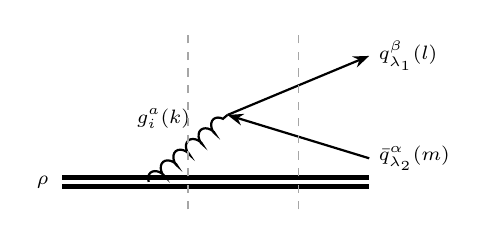
\begin{tikzpicture}
\draw[val] (0,0) -- (3.9,0); \node[left] at (-0.05,0) {\scriptsize$\rho$};
\draw[gl] (1.1,0) -- (2.1,0.85); \node[above left] at (1.75,0.55) {\scriptsize$\gl{a}{i}{k}$};
\draw[qk] (2.1,0.85) -- (3.9,1.6); \node[right] at (3.9,1.6) {\scriptsize$\qk{\beta}{\lambda_{1}}{l}$};
\draw[qk] (3.9,0.3) -- (2.1,0.85); \node[right] at (3.9,0.3) {\scriptsize$\aqk{\alpha}{\lambda_{2}}{m}$};
\draw[cut] (1.6,-0.35) -- (1.6,1.95); \draw[cut] (3.0,-0.35) -- (3.0,1.95);
\end{tikzpicture}
\end{center}
\begin{equation}
\ket{\Psi^{1}_{q\bar q}}=\sum_{\lambda_{1}\lambda_{2},f}\int\! d^{3}k\,d^{3}l\,d^{3}m\;
\ket{\qk{\beta}{\lambda_{1}}{l}\aqk{\alpha}{\lambda_{2}}{m}}\;
\frac{\bra{\qk{\beta}{\lambda_{1}}{l}\aqk{\alpha}{\lambda_{2}}{m}}H_{gq\bar q}\ket{\gl{a}{i}{k}}}
{E_{q\bar q}(l,m)}\;
\frac{\bra{\gl{a}{i}{k}}H_{g}\vac}{E_{g}(k)}
\end{equation}
Using the matrix elements \eqref{eq:MEqqg} and \eqref{eq:MEg}, and $k=l+m$,
\begin{equation}
\ket{\Psi^{1}_{q\bar q}}=\frac{g^{2}}{32\pi^{3}}\sum_{\lambda_{1}\lambda_{2},f}\int\!d^{3}l\,d^{3}m\;
\ket{\qk{\beta}{\lambda_{1}}{l}\aqk{\alpha}{\lambda_{2}}{m}}\;
\frac{t^{a}_{\beta\alpha}\,\rho^{a}(-k)\,k^{i}\,\Ph^{i}_{\lambda_{1}\lambda_{2}}(k;l,m)}
{(k^{+})^{2}\,\eps_{k}\,\big(\eps_{l}+\eps_{m}\big)} .
\label{eq:P1}
\end{equation}

\paragraph{(b) Instantaneous gluon exchange with the valence.}
\begin{center}
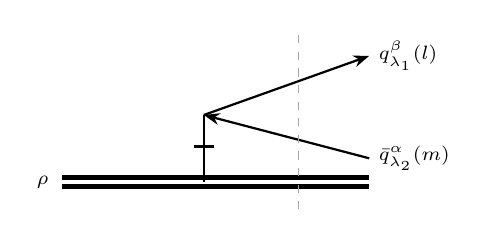
\begin{tikzpicture}
\draw[val] (0,0) -- (3.9,0); \node[left] at (-0.05,0) {\scriptsize$\rho$};
\draw[ins] (1.8,0) -- (1.8,0.85); \ibar{1.8}{0.45}
\draw[qk] (1.8,0.85) -- (3.9,1.6); \node[right] at (3.9,1.6) {\scriptsize$\qk{\beta}{\lambda_{1}}{l}$};
\draw[qk] (3.9,0.3) -- (1.8,0.85); \node[right] at (3.9,0.3) {\scriptsize$\aqk{\alpha}{\lambda_{2}}{m}$};
\draw[cut] (3.0,-0.35) -- (3.0,1.95);
\end{tikzpicture}
\end{center}
\begin{equation}
\ket{\Psi^{2}_{q\bar q}}=-\sum_{\lambda_{1}\lambda_{2},f}\int\! d^{3}l\,d^{3}m\;
\ket{\qk{\beta}{\lambda_{1}}{l}\aqk{\alpha}{\lambda_{2}}{m}}\;
\frac{\bra{\qk{\beta}{\lambda_{1}}{l}\aqk{\alpha}{\lambda_{2}}{m}}H_{q\bar q-\rm inst}\vac}
{E_{q\bar q}(l,m)}
\end{equation}
\begin{equation}
\ket{\Psi^{2}_{q\bar q}}=-\frac{g^{2}}{8\pi^{3}}\sum_{\lambda_{1}\lambda_{2},f}\int\!d^{3}l\,d^{3}m\;
\ket{\qk{\beta}{\lambda_{1}}{l}\aqk{\alpha}{\lambda_{2}}{m}}\;
\frac{t^{a}_{\beta\alpha}\,\rho^{a}(-k)\,\delta_{\lambda_{1}\lambda_{2}}}
{(k^{+})^{2}\,\big(\eps_{l}+\eps_{m}\big)} .
\label{eq:P2}
\end{equation}

%------------------------------------------------------------------
\subsection{Single-gluon incoming state}
%------------------------------------------------------------------
\subsubsection{Quark and antiquark outgoing}

\paragraph{($\rho$ independent) The incoming gluon splits into a pair.}
\begin{center}
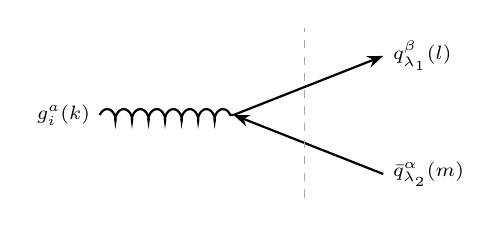
\begin{tikzpicture}
\draw[gl] (0,0.85) -- (1.7,0.85); \node[left] at (0,0.85) {\scriptsize$\gl{a}{i}{k}$};
\draw[qk] (1.7,0.85) -- (3.6,1.6); \node[right] at (3.6,1.6) {\scriptsize$\qk{\beta}{\lambda_{1}}{l}$};
\draw[qk] (3.6,0.1) -- (1.7,0.85); \node[right] at (3.6,0.1) {\scriptsize$\aqk{\alpha}{\lambda_{2}}{m}$};
\draw[cut] (2.6,-0.2) -- (2.6,1.95);
\end{tikzpicture}
\end{center}
\begin{equation}
\ket{\Psi^{a}_{i}(k)_{q\bar q}}=\sum_{\lambda_{1}\lambda_{2},f}\int\! d^{3}l\,d^{3}m\;
\ket{\qk{\beta}{\lambda_{1}}{l}\aqk{\alpha}{\lambda_{2}}{m}}\;
\frac{\bra{\qk{\beta}{\lambda_{1}}{l}\aqk{\alpha}{\lambda_{2}}{m}}H_{gq\bar q}\ket{\gl{a}{i}{k}}}
{E_{g}(k)-E_{q\bar q}(l,m)}
\end{equation}
\begin{equation}
\ket{\Psi^{a}_{i}(k)_{q\bar q}}=\frac{g}{8\pi^{3/2}}\sum_{\lambda_{1}\lambda_{2},f}
\int\! d^{3}l\,d^{3}m\;\ket{\qk{\beta}{\lambda_{1}}{l}\aqk{\alpha}{\lambda_{2}}{m}}\;
\frac{t^{a}_{\beta\alpha}\,\dthree(k-l-m)\,\Ph^{i}_{\lambda_{1}\lambda_{2}}(k;l,m)}
{\sqrt{k^{+}}\;\big(\eps_{k}-\eps_{l}-\eps_{m}\big)\chg{17}}
\label{eq:Pg}
\end{equation}

\subsubsection{One gluon, quark and antiquark outgoing}

There are seven connected contributions. Throughout the outgoing gluon is $\gl{d}{n}{r}$ and
\begin{equation}
D_{f}\equiv\eps_{k}-\eps_{l}-\eps_{m}-\eps_{r} .
\end{equation}

\paragraph{(a) The gluon splits, then the quark emits ($\rho$ independent).}
\begin{center}
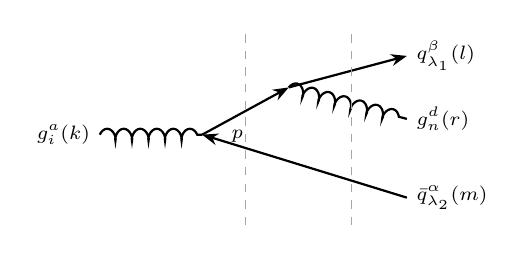
\begin{tikzpicture}
\draw[gl] (0,0.9) -- (1.3,0.9); \node[left] at (0,0.9) {\scriptsize$\gl{a}{i}{k}$};
\draw[qk] (1.3,0.9) -- (2.4,1.5); \node[below right] at (1.55,1.08) {\scriptsize$p$};
\draw[qk] (2.4,1.5) -- (3.9,1.9); \node[right] at (3.9,1.9) {\scriptsize$\qk{\beta}{\lambda_{1}}{l}$};
\draw[gl] (2.4,1.5) -- (3.9,1.1); \node[right] at (3.9,1.1) {\scriptsize$\gl{d}{n}{r}$};
\draw[qk] (3.9,0.1) -- (1.3,0.9); \node[right] at (3.9,0.1) {\scriptsize$\aqk{\alpha}{\lambda_{2}}{m}$};
\draw[cut] (1.85,-0.25) -- (1.85,2.25); \draw[cut] (3.2,-0.25) -- (3.2,2.25);
\end{tikzpicture}
\end{center}
\begin{align}
\ket{\Psi^{a}_{i}(k)^{1}_{gq\bar q}}=\sum\int\! d^{3}p\,d^{3}l\,d^{3}m\,d^{3}r\;
&\ket{\qk{\beta}{\lambda_{1}}{l}\aqk{\alpha}{\lambda_{2}}{m}\gl{d}{n}{r}}
\nonumber\\&\times
\frac{\bra{\qk{\beta}{\lambda_{1}}{l}\gl{d}{n}{r}}H_{gq\bar q}\ket{\qk{\gamma}{\lambda}{p}}}
{E_{g}(k)-E_{g}(r)-E_{q\bar q}(l,m)}\;
\frac{\bra{\qk{\gamma}{\lambda}{p}\aqk{\alpha}{\lambda_{2}}{m}}H_{gq\bar q}\ket{\gl{a}{i}{k}}}
{E_{g}(k)-E_{q\bar q}(p,m)}
\end{align}
Using \eqref{eq:MEqqg} and \eqref{eq:MEqg}, closing the intermediate helicity sum with
$\sum_{\lambda}\chi_{\lambda}\chi^{\dg}_{\lambda}=\mathbf{1}$, and $p=l+r$,
\begin{align}
\ket{\Psi^{a}_{i}(k)^{1}_{gq\bar q}}=\frac{g^{2}}{64\pi^{3}}\sum\int\! d^{3}l\,d^{3}m\,d^{3}r\;
&\ket{\qk{\beta}{\lambda_{1}}{l}\aqk{\alpha}{\lambda_{2}}{m}\gl{d}{n}{r}}\,
(t^{d}t^{a})_{\beta\alpha}\,\frac{\dthree(k-l-m-r)}{\sqrt{r^{+}k^{+}}}
\nonumber\\&\times
\frac{\chi^{\dg}_{\lambda_{1}}\Gam^{n}(r;l,p)\chg{18}\,\Gam^{i}(k;p,m)\chi_{\lambda_{2}}}
{D_{f}\,\big(\eps_{k}-\eps_{p}-\eps_{m}\big)}
\label{eq:B2a}
\end{align}

\paragraph{(b) The gluon splits, then the antiquark emits ($\rho$ independent).}
\begin{center}
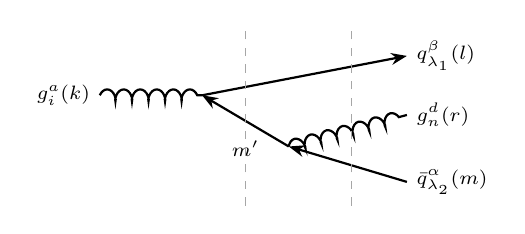
\begin{tikzpicture}
\draw[gl] (0,1.6) -- (1.3,1.6); \node[left] at (0,1.6) {\scriptsize$\gl{a}{i}{k}$};
\draw[qk] (1.3,1.6) -- (3.9,2.1); \node[right] at (3.9,2.1) {\scriptsize$\qk{\beta}{\lambda_{1}}{l}$};
\draw[qk] (2.4,0.95) -- (1.3,1.6); \node[below] at (1.85,1.15) {\scriptsize$m'$};
\draw[qk] (3.9,0.5) -- (2.4,0.95); \node[right] at (3.9,0.5) {\scriptsize$\aqk{\alpha}{\lambda_{2}}{m}$};
\draw[gl] (2.4,0.95) -- (3.9,1.35); \node[right] at (3.9,1.35) {\scriptsize$\gl{d}{n}{r}$};
\draw[cut] (1.85,0.2) -- (1.85,2.45); \draw[cut] (3.2,0.2) -- (3.2,2.45);
\end{tikzpicture}
\end{center}
\begin{align}
\ket{\Psi^{a}_{i}(k)^{2}_{gq\bar q}}=\sum\int\! d^{3}m'\,d^{3}l\,d^{3}m\,d^{3}r\;
&\ket{\qk{\beta}{\lambda_{1}}{l}\aqk{\alpha}{\lambda_{2}}{m}\gl{d}{n}{r}}
\nonumber\\&\times
\frac{\bra{\aqk{\alpha}{\lambda_{2}}{m}\gl{d}{n}{r}}H_{gq\bar q}\ket{\aqk{\alpha'}{\lambda}{m'}}}
{E_{g}(k)-E_{g}(r)-E_{q\bar q}(l,m)}\;
\frac{\bra{\qk{\beta}{\lambda_{1}}{l}\aqk{\alpha'}{\lambda}{m'}}H_{gq\bar q}\ket{\gl{a}{i}{k}}}
{E_{g}(k)-E_{q\bar q}(l,m')}
\end{align}
With $m'=m+r$, and the minus sign and transposed colour matrix of the antiquark vertex
\eqref{eq:MEaqg},
\begin{align}
\ket{\Psi^{a}_{i}(k)^{2}_{gq\bar q}}=-\frac{g^{2}}{64\pi^{3}}\sum\int\! d^{3}l\,d^{3}m\,d^{3}r\;
&\ket{\qk{\beta}{\lambda_{1}}{l}\aqk{\alpha}{\lambda_{2}}{m}\gl{d}{n}{r}}\,
(t^{a}t^{d})_{\beta\alpha}\,\frac{\dthree(k-l-m-r)}{\sqrt{r^{+}k^{+}}}
\nonumber\\&\times
\frac{\chi^{\dg}_{\lambda_{1}}\Gam^{i}(k;l,m')\,\Gam^{n}(r;m',m)\chg{18}\chi_{\lambda_{2}}}
{D_{f}\,\big(\eps_{k}-\eps_{l}-\eps_{m'}\big)}
\label{eq:B2b}
\end{align}

\paragraph{(c) The gluon splits into two gluons, one of which splits into a pair
($\rho$ independent).\chg{19}}
\begin{center}
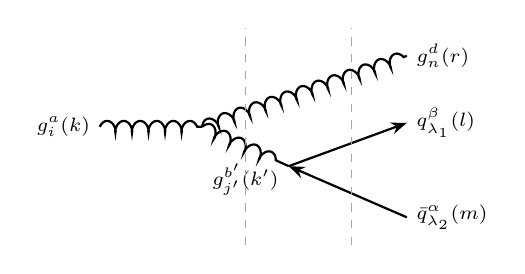
\begin{tikzpicture}
\draw[gl] (0,1.1) -- (1.3,1.1); \node[left] at (0,1.1) {\scriptsize$\gl{a}{i}{k}$};
\draw[gl] (1.3,1.1) -- (3.9,2.0); \node[right] at (3.9,2.0) {\scriptsize$\gl{d}{n}{r}$};
\draw[gl] (1.3,1.1) -- (2.4,0.6); \node[below] at (1.85,0.75) {\scriptsize$\gl{b'}{j'}{k'}$};
\draw[qk] (2.4,0.6) -- (3.9,1.15); \node[right] at (3.9,1.15) {\scriptsize$\qk{\beta}{\lambda_{1}}{l}$};
\draw[qk] (3.9,-0.05) -- (2.4,0.6); \node[right] at (3.9,-0.05) {\scriptsize$\aqk{\alpha}{\lambda_{2}}{m}$};
\draw[cut] (1.85,-0.4) -- (1.85,2.35); \draw[cut] (3.2,-0.4) -- (3.2,2.35);
\end{tikzpicture}
\end{center}
\begin{align}
\ket{\Psi^{a}_{i}(k)^{3}_{gq\bar q}}=\frac12\sum\int\! d^{3}k'\,d^{3}l\,d^{3}m\,d^{3}r\;
&\ket{\qk{\beta}{\lambda_{1}}{l}\aqk{\alpha}{\lambda_{2}}{m}\gl{d}{n}{r}}
\nonumber\\&\times
\frac{\bra{\qk{\beta}{\lambda_{1}}{l}\aqk{\alpha}{\lambda_{2}}{m}}H_{gq\bar q}\ket{\gl{b'}{j'}{k'}}}
{E_{g}(k)-E_{g}(r)-E_{q\bar q}(l,m)}\;
\frac{\bra{\gl{b'}{j'}{k'}\gl{d}{n}{r}}H_{ggg}\ket{\gl{a}{i}{k}}}
{E_{g}(k)-E_{gg}(k',r)}
\end{align}
The $\tfrac12$ cancels against the two assignments of the intermediate gluon pair. With $k'=l+m$,
\begin{align}
\ket{\Psi^{a}_{i}(k)^{3}_{gq\bar q}}=\frac{ig^{2}}{64\pi^{3}}\sum\int\! d^{3}l\,d^{3}m\,d^{3}r\;
&\ket{\qk{\beta}{\lambda_{1}}{l}\aqk{\alpha}{\lambda_{2}}{m}\gl{d}{n}{r}}\,
f^{ab'd}t^{b'}_{\beta\alpha}\,\frac{\dthree(k-l-m-r)}{k'^{+}\sqrt{k^{+}r^{+}}}
\nonumber\\&\times
\frac{\Vg^{ij'n}(k;k',r)\;\Ph^{j'}_{\lambda_{1}\lambda_{2}}(k';l,m)}
{D_{f}\,\big(\eps_{k}-\eps_{k'}-\eps_{r}\big)}
\label{eq:B2c}
\end{align}

\paragraph{(d), (e) The valence emits the gluon $r$ and the incoming gluon splits: two orderings.}
\begin{center}
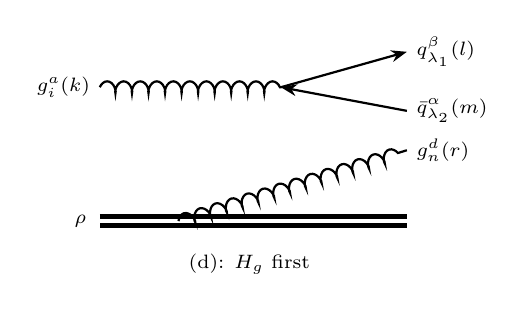
\begin{tikzpicture}
\draw[val] (0,0) -- (3.9,0); \node[left] at (-0.05,0) {\scriptsize$\rho$};
\draw[gl] (0,1.7) -- (2.3,1.7); \node[left] at (0,1.7) {\scriptsize$\gl{a}{i}{k}$};
\draw[gl] (1.0,0) -- (3.9,0.9); \node[right] at (3.9,0.9) {\scriptsize$\gl{d}{n}{r}$};
\draw[qk] (2.3,1.7) -- (3.9,2.15); \node[right] at (3.9,2.15) {\scriptsize$\qk{\beta}{\lambda_{1}}{l}$};
\draw[qk] (3.9,1.4) -- (2.3,1.7); \node[right] at (3.9,1.4) {\scriptsize$\aqk{\alpha}{\lambda_{2}}{m}$};
\node at (1.9,-0.55) {\scriptsize (d): $H_{g}$ first};
\end{tikzpicture}
\hspace{0.7cm}
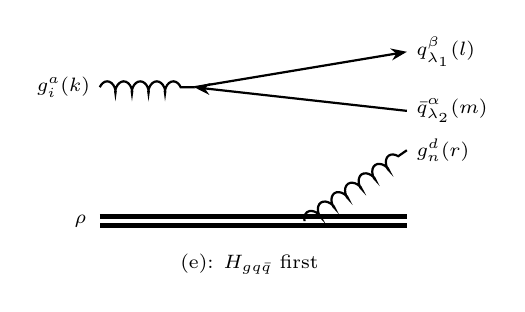
\begin{tikzpicture}
\draw[val] (0,0) -- (3.9,0); \node[left] at (-0.05,0) {\scriptsize$\rho$};
\draw[gl] (0,1.7) -- (1.2,1.7); \node[left] at (0,1.7) {\scriptsize$\gl{a}{i}{k}$};
\draw[gl] (2.6,0) -- (3.9,0.9); \node[right] at (3.9,0.9) {\scriptsize$\gl{d}{n}{r}$};
\draw[qk] (1.2,1.7) -- (3.9,2.15); \node[right] at (3.9,2.15) {\scriptsize$\qk{\beta}{\lambda_{1}}{l}$};
\draw[qk] (3.9,1.4) -- (1.2,1.7); \node[right] at (3.9,1.4) {\scriptsize$\aqk{\alpha}{\lambda_{2}}{m}$};
\node at (1.9,-0.55) {\scriptsize (e): $H_{gq\bar q}$ first};
\end{tikzpicture}
\end{center}
In (d) the valence emits first, so the intermediate state is
$\ket{\gl{a}{i}{k}\gl{d}{n}{r}}$ and the denominator is $E_{g}(k)-E_{gg}(k,r)=-\eps_{r}$. In (e)
the pair is formed first and the intermediate state is
$\ket{\qk{\beta}{\lambda_{1}}{l}\aqk{\alpha}{\lambda_{2}}{m}}$:
\begin{align}
\ket{\Psi^{a}_{i}(k)^{4}_{gq\bar q}}&=\sum\int\!d^{3}l\,d^{3}m\,d^{3}r\;
\ket{q\bar q\,\gl{d}{n}{r}}\;
\frac{\bra{q\bar q\,\gl{d}{n}{r}}H_{gq\bar q}\ket{\gl{a}{i}{k}\gl{d}{n}{r}}}{D_{f}}\;
\frac{\bra{\gl{a}{i}{k}\gl{d}{n}{r}}H_{g}\ket{\gl{a}{i}{k}}}{-\eps_{r}}\chg{20}
\\
\ket{\Psi^{a}_{i}(k)^{5}_{gq\bar q}}&=\sum\int\!d^{3}l\,d^{3}m\,d^{3}r\;
\ket{q\bar q\,\gl{d}{n}{r}}\;
\frac{\bra{q\bar q\,\gl{d}{n}{r}}H_{g}\ket{q\bar q}}{D_{f}}\;
\frac{\bra{q\bar q}H_{gq\bar q}\ket{\gl{a}{i}{k}}}{\eps_{k}-\eps_{l}-\eps_{m}}
\end{align}
Their sum is
\begin{align}
\ket{\Psi^{a}_{i}(k)^{4+5}_{gq\bar q}}=\frac{g^{2}}{32\pi^{3}}\sum\int\!d^{3}l\,d^{3}m\,d^{3}r\;
&\ket{\qk{\beta}{\lambda_{1}}{l}\aqk{\alpha}{\lambda_{2}}{m}\gl{d}{n}{r}}\;
\frac{t^{a}_{\beta\alpha}\,r^{n}\,\Ph^{i}_{\lambda_{1}\lambda_{2}}(k;l,m)\,\dthree(k-l-m)}
{\sqrt{k^{+}}(r^{+})^{3/2}\,D_{f}}
\nonumber\\&\times
\left[\frac{\rho^{d}(-r)}{\eps_{k}-\eps_{l}-\eps_{m}}-\frac{\rho^{d}(-r)}{\eps_{r}}\right]
\label{eq:B2de}
\end{align}
where in the first (second) term $H_{g}$ acts last (first); $t^{a}$ is a numerical matrix, so its
ordering relative to $\rho^{d}$ is immaterial, but it is displayed for bookkeeping.

\paragraph{(f) Instantaneous quark exchange.\chg{21}}
\begin{center}
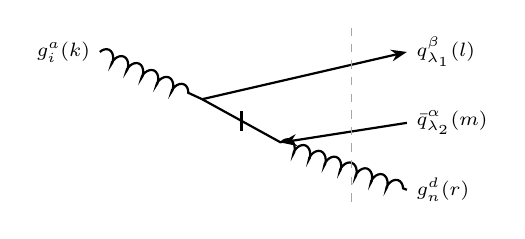
\begin{tikzpicture}
\draw[gl] (0,1.9) -- (1.3,1.3); \node[left] at (0,1.9) {\scriptsize$\gl{a}{i}{k}$};
\draw[gl] (2.3,0.75) -- (3.9,0.15); \node[right] at (3.9,0.15) {\scriptsize$\gl{d}{n}{r}$};
\draw[qk] (1.3,1.3) -- (3.9,1.9); \node[right] at (3.9,1.9) {\scriptsize$\qk{\beta}{\lambda_{1}}{l}$};
\draw[ins] (1.3,1.3) -- (2.3,0.75); \ibarh{1.8}{1.025}
\draw[qk] (3.9,1.0) -- (2.3,0.75); \node[right] at (3.9,1.0) {\scriptsize$\aqk{\alpha}{\lambda_{2}}{m}$};
\draw[cut] (3.2,0.0) -- (3.2,2.2);
\end{tikzpicture}
\end{center}
\begin{equation}
\ket{\Psi^{a}_{i}(k)^{6}_{gq\bar q}}=\sum\int\!d^{3}l\,d^{3}m\,d^{3}r\;
\ket{q\bar q\,\gl{d}{n}{r}}\;
\frac{\bra{\qk{\beta}{\lambda_{1}}{l}\aqk{\alpha}{\lambda_{2}}{m}\gl{d}{n}{r}}
H_{ggq\bar q}\ket{\gl{a}{i}{k}}}{D_{f}}
\end{equation}
The two orderings of the gluon attachments give instantaneous longitudinal momenta
$P^{+}_{\rm inst}=l^{+}+r^{+}$ and $-(m^{+}+r^{+})$:
\begin{align}
\ket{\Psi^{a}_{i}(k)^{6}_{gq\bar q}}=\frac{g^{2}}{16\pi^{3}}\sum\int\!d^{3}l\,d^{3}m\,d^{3}r\;
&\ket{\qk{\beta}{\lambda_{1}}{l}\aqk{\alpha}{\lambda_{2}}{m}\gl{d}{n}{r}}\,
\frac{\dthree(k-l-m-r)}{\sqrt{k^{+}r^{+}}\,D_{f}}
\nonumber\\&\times
\chi^{\dg}_{\lambda_{1}}\!\left[\frac{(t^{d}t^{a})_{\beta\alpha}\sigma^{n}\sigma^{i}}{l^{+}+r^{+}}
-\frac{(t^{a}t^{d})_{\beta\alpha}\sigma^{i}\sigma^{n}}{m^{+}+r^{+}}\right]\chi_{\lambda_{2}}
\label{eq:B2f}
\end{align}

\paragraph{(g) Instantaneous gluon exchange between the soft gluon and the soft quark
current.\chg{35}}
\begin{center}
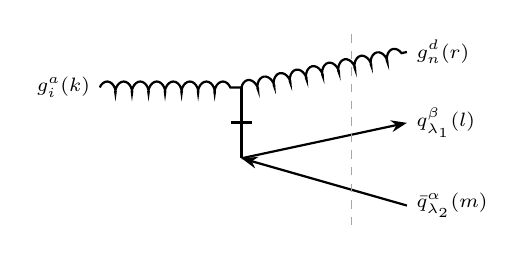
\begin{tikzpicture}
\draw[gl] (0,1.6) -- (1.8,1.6); \node[left] at (0,1.6) {\scriptsize$\gl{a}{i}{k}$};
\draw[gl] (1.8,1.6) -- (3.9,2.05); \node[right] at (3.9,2.05) {\scriptsize$\gl{d}{n}{r}$};
\draw[ins] (1.8,1.6) -- (1.8,0.7); \ibar{1.8}{1.15}
\draw[qk] (1.8,0.7) -- (3.9,1.15); \node[right] at (3.9,1.15) {\scriptsize$\qk{\beta}{\lambda_{1}}{l}$};
\draw[qk] (3.9,0.1) -- (1.8,0.7); \node[right] at (3.9,0.1) {\scriptsize$\aqk{\alpha}{\lambda_{2}}{m}$};
\draw[cut] (3.2,-0.15) -- (3.2,2.35);
\end{tikzpicture}
\end{center}
This is the $\Jc_{q}\!\cdot\!\Jc_{g}$ cross term of $H^{(A)}_{\rm inst}$, Eq.~\eqref{eq:HinstA}.
The instantaneous gluon carries $P^{+}=l^{+}+m^{+}=k^{+}-r^{+}$:
\begin{equation}
\ket{\Psi^{a}_{i}(k)^{7}_{gq\bar q}}=\sum\int\!d^{3}l\,d^{3}m\,d^{3}r\;
\ket{q\bar q\,\gl{d}{n}{r}}\;
\frac{\bra{\qk{\beta}{\lambda_{1}}{l}\aqk{\alpha}{\lambda_{2}}{m}\gl{d}{n}{r}}
H^{(A)}_{\rm inst}\ket{\gl{a}{i}{k}}}{D_{f}}
\end{equation}
\begin{align}
\ket{\Psi^{a}_{i}(k)^{7}_{gq\bar q}}=\frac{i g^{2}}{2(2\pi)^{3}}\sum\int\!d^{3}l\,d^{3}m\,d^{3}r\;
&\ket{\qk{\beta}{\lambda_{1}}{l}\aqk{\alpha}{\lambda_{2}}{m}\gl{d}{n}{r}}
\nonumber\\&\times
\frac{f^{bad}\,t^{b}_{\beta\alpha}\,\delta_{\lambda_{1}\lambda_{2}}\,\delta_{in}\,(k^{+}+r^{+})\,
\dthree(k-l-m-r)}{\sqrt{k^{+}r^{+}}\,(l^{+}+m^{+})^{2}\,D_{f}}
\label{eq:B2g}
\end{align}

\paragraph{Disconnected.\chg{22}} The remaining topology --- the valence emits a gluon which then
splits, the incoming gluon $\gl{a}{i}{k}$ remaining a spectator --- is disconnected. It is the
$\A_{1}$ term of Eq.~\eqref{eq:Omg} and must be subtracted, not added, when $\B_{3}$ is read off.

%------------------------------------------------------------------
\subsection{Two-gluon incoming state}
%------------------------------------------------------------------
\subsubsection{Quark and antiquark outgoing}

Incoming $\gl{a}{i}{k}\gl{b}{j}{p}$; here
\begin{equation}
D_{f}\equiv\eps_{k}+\eps_{p}-\eps_{l}-\eps_{m},
\end{equation}
and every expression is understood with $+\,(k\leftrightarrow p)$, supplied by the symmetrization
in Eq.~\eqref{eq:Omgg}.

\paragraph{(a) The two gluons merge; the resulting gluon splits ($\rho$ independent).}
\begin{center}
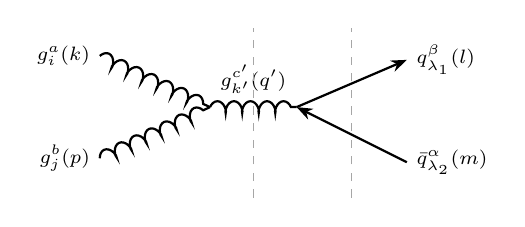
\begin{tikzpicture}
\draw[gl] (0,1.9) -- (1.4,1.25); \node[left] at (0,1.9) {\scriptsize$\gl{a}{i}{k}$};
\draw[gl] (0,0.6) -- (1.4,1.25); \node[left] at (0,0.6) {\scriptsize$\gl{b}{j}{p}$};
\draw[gl] (1.4,1.25) -- (2.5,1.25); \node[above] at (1.95,1.3) {\scriptsize$\gl{c'}{k'}{q'}$};
\draw[qk] (2.5,1.25) -- (3.9,1.85); \node[right] at (3.9,1.85) {\scriptsize$\qk{\beta}{\lambda_{1}}{l}$};
\draw[qk] (3.9,0.55) -- (2.5,1.25); \node[right] at (3.9,0.55) {\scriptsize$\aqk{\alpha}{\lambda_{2}}{m}$};
\draw[cut] (1.95,0.1) -- (1.95,2.25); \draw[cut] (3.2,0.1) -- (3.2,2.25);
\end{tikzpicture}
\end{center}
\begin{equation}
\ket{\Psi^{ba}_{ji}(k,p)^{1}_{q\bar q}}=\sum\int\! d^{3}q'\,d^{3}l\,d^{3}m\;
\ket{q\bar q}\;
\frac{\bra{\qk{\beta}{\lambda_{1}}{l}\aqk{\alpha}{\lambda_{2}}{m}}H_{gq\bar q}\ket{\gl{c'}{k'}{q'}}}
{D_{f}}\;
\frac{\bra{\gl{c'}{k'}{q'}}H_{ggg}\ket{\gl{a}{i}{k}\gl{b}{j}{p}}}{E_{gg}(k,p)-E_{g}(q')}
\end{equation}
With $q'\equiv k'=k+p$, and noting that the $2\to1$ gluon vertex is the Hermitian conjugate of
\eqref{eq:MEggg},
\begin{align}
\ket{\Psi^{ba}_{ji}(k,p)^{1}_{q\bar q}}=-\frac{ig^{2}}{64\pi^{3}}\sum\int\!d^{3}l\,d^{3}m\;
&\ket{\qk{\beta}{\lambda_{1}}{l}\aqk{\alpha}{\lambda_{2}}{m}}\,f^{abc'}t^{c'}_{\beta\alpha}\,
\frac{\dthree(k+p-l-m)}{k'^{+}\chg{23}\sqrt{k^{+}p^{+}}}
\nonumber\\&\times
\frac{\Vg^{k'ij}(k';k,p)\;\Ph^{k'}_{\lambda_{1}\lambda_{2}}(k';l,m)}
{\big(\eps_{k}+\eps_{p}-\eps_{k'}\big)\,D_{f}}+(k\leftrightarrow p)
\label{eq:C1a}
\end{align}

\paragraph{(b) One gluon is absorbed by the valence, the other splits: two orderings.}
\begin{center}
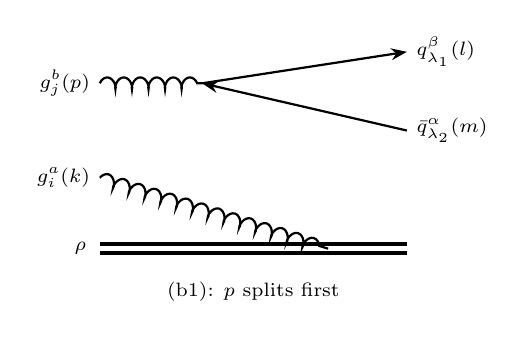
\begin{tikzpicture}
\draw[val] (0,0) -- (3.9,0); \node[left] at (-0.05,0) {\scriptsize$\rho$};
\draw[gl] (0,0.9) -- (2.9,0); \node[left] at (0,0.9) {\scriptsize$\gl{a}{i}{k}$};
\draw[gl] (0,2.1) -- (1.3,2.1); \node[left] at (0,2.1) {\scriptsize$\gl{b}{j}{p}$};
\draw[qk] (1.3,2.1) -- (3.9,2.5); \node[right] at (3.9,2.5) {\scriptsize$\qk{\beta}{\lambda_{1}}{l}$};
\draw[qk] (3.9,1.5) -- (1.3,2.1); \node[right] at (3.9,1.5) {\scriptsize$\aqk{\alpha}{\lambda_{2}}{m}$};
\node at (1.95,-0.55) {\scriptsize (b1): $p$ splits first};
\end{tikzpicture}
\hspace{0.5cm}
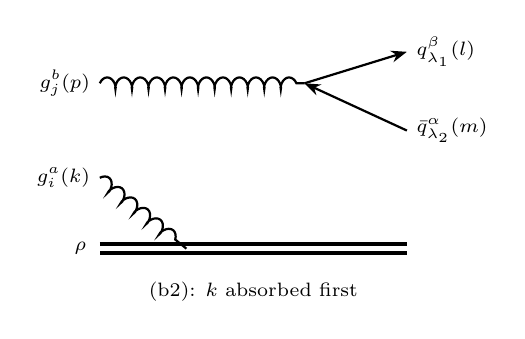
\begin{tikzpicture}
\draw[val] (0,0) -- (3.9,0); \node[left] at (-0.05,0) {\scriptsize$\rho$};
\draw[gl] (0,0.9) -- (1.1,0); \node[left] at (0,0.9) {\scriptsize$\gl{a}{i}{k}$};
\draw[gl] (0,2.1) -- (2.6,2.1); \node[left] at (0,2.1) {\scriptsize$\gl{b}{j}{p}$};
\draw[qk] (2.6,2.1) -- (3.9,2.5); \node[right] at (3.9,2.5) {\scriptsize$\qk{\beta}{\lambda_{1}}{l}$};
\draw[qk] (3.9,1.5) -- (2.6,2.1); \node[right] at (3.9,1.5) {\scriptsize$\aqk{\alpha}{\lambda_{2}}{m}$};
\node at (1.95,-0.55) {\scriptsize (b2): $k$ absorbed first};
\end{tikzpicture}
\end{center}
In (b1) the intermediate state is $\ket{q\bar q\,\gl{a}{i}{k}}$, giving
$E_{gg}(k,p)-\eps_{k}-\eps_{l}-\eps_{m}=\eps_{p}-\eps_{l}-\eps_{m}$; in (b2) it is
$\ket{\gl{b}{j}{p}}$, giving $E_{gg}(k,p)-\eps_{p}=\eps_{k}$:
\begin{align}
\ket{\Psi^{ba}_{ji}(k,p)^{2}_{q\bar q}}&=\sum\int\!d^{3}l\,d^{3}m\;\ket{q\bar q}\;
\frac{\bra{q\bar q}H_{g}\ket{q\bar q\,\gl{a}{i}{k}}}{D_{f}}\;
\frac{\bra{q\bar q\,\gl{a}{i}{k}}H_{gq\bar q}\ket{\gl{a}{i}{k}\gl{b}{j}{p}}}
{\eps_{p}-\eps_{l}-\eps_{m}}
\\
\ket{\Psi^{ba}_{ji}(k,p)^{3}_{q\bar q}}&=\sum\int\!d^{3}l\,d^{3}m\;\ket{q\bar q}\;
\frac{\bra{q\bar q}H_{gq\bar q}\ket{\gl{b}{j}{p}}}{D_{f}}\;
\frac{\bra{\gl{b}{j}{p}}H_{g}\ket{\gl{a}{i}{k}\gl{b}{j}{p}}}{\eps_{k}}
\end{align}
which evaluate to
\begin{align}
\ket{\Psi^{ba}_{ji}(k,p)^{2}_{q\bar q}}&=\frac{g^{2}}{32\pi^{3}}\sum\int\!d^{3}l\,d^{3}m\;
\ket{q\bar q}\;
\frac{\rho^{a}(k)\,t^{b}_{\beta\alpha}\,k^{i}\,\Ph^{j}_{\lambda_{1}\lambda_{2}}(p;l,m)\,
\dthree(p-l-m)}
{(k^{+})^{3/2}\sqrt{p^{+}}\,\big(\eps_{p}-\eps_{l}-\eps_{m}\big)\,D_{f}\chg{24}}+(k\leftrightarrow p)
\label{eq:C1b1}\\
\ket{\Psi^{ba}_{ji}(k,p)^{3}_{q\bar q}}&=\frac{g^{2}}{16\pi^{3}}\chg{25}
\sum\int\!d^{3}l\,d^{3}m\;\ket{q\bar q}\;
\frac{t^{b}_{\beta\alpha}\,\rho^{a}(k)\,k^{i}\,\Ph^{j}_{\lambda_{1}\lambda_{2}}(p;l,m)\,
\dthree(p-l-m)}{\sqrt{k^{+}p^{+}}\;k^{2}\;D_{f}}+(k\leftrightarrow p)
\label{eq:C1b2}
\end{align}

\paragraph{(c) Instantaneous quark exchange.\chg{26}}
\begin{center}
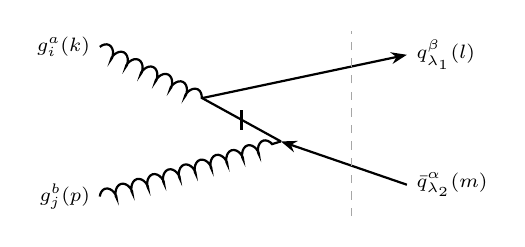
\begin{tikzpicture}
\draw[gl] (0,2.0) -- (1.3,1.35); \node[left] at (0,2.0) {\scriptsize$\gl{a}{i}{k}$};
\draw[gl] (0,0.1) -- (2.3,0.8); \node[left] at (0,0.1) {\scriptsize$\gl{b}{j}{p}$};
\draw[qk] (1.3,1.35) -- (3.9,1.9); \node[right] at (3.9,1.9) {\scriptsize$\qk{\beta}{\lambda_{1}}{l}$};
\draw[ins] (1.3,1.35) -- (2.3,0.8); \ibarh{1.8}{1.075}
\draw[qk] (3.9,0.25) -- (2.3,0.8); \node[right] at (3.9,0.25) {\scriptsize$\aqk{\alpha}{\lambda_{2}}{m}$};
\draw[cut] (3.2,-0.15) -- (3.2,2.2);
\end{tikzpicture}
\end{center}
\begin{align}
\ket{\Psi^{ba}_{ji}(k,p)^{4}_{q\bar q}}=\frac{g^{2}}{16\pi^{3}}\sum\int\!d^{3}l\,d^{3}m\;
&\ket{\qk{\beta}{\lambda_{1}}{l}\aqk{\alpha}{\lambda_{2}}{m}}\,
\frac{\dthree(k+p-l-m)}{\sqrt{k^{+}p^{+}}\,D_{f}}
\nonumber\\&\times
\chi^{\dg}_{\lambda_{1}}\!\left[\frac{(t^{a}t^{b})_{\beta\alpha}\sigma^{i}\sigma^{j}}{l^{+}-k^{+}}
+\frac{(t^{b}t^{a})_{\beta\alpha}\sigma^{j}\sigma^{i}}{l^{+}-p^{+}}\right]\chi_{\lambda_{2}}
\label{eq:C1c}
\end{align}

\paragraph{(d) Instantaneous gluon exchange, $\Jc_{q}\!\cdot\!\Jc_{g}$.\chg{35}}
\begin{center}
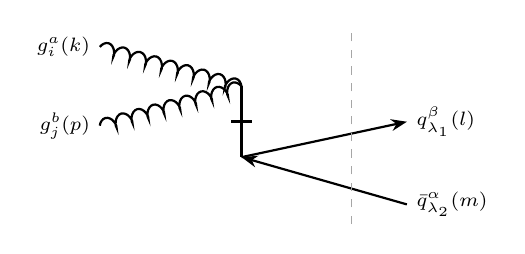
\begin{tikzpicture}
\draw[gl] (0,2.0) -- (1.8,1.5); \node[left] at (0,2.0) {\scriptsize$\gl{a}{i}{k}$};
\draw[gl] (0,1.0) -- (1.8,1.5); \node[left] at (0,1.0) {\scriptsize$\gl{b}{j}{p}$};
\draw[ins] (1.8,1.5) -- (1.8,0.6); \ibar{1.8}{1.05}
\draw[qk] (1.8,0.6) -- (3.9,1.05); \node[right] at (3.9,1.05) {\scriptsize$\qk{\beta}{\lambda_{1}}{l}$};
\draw[qk] (3.9,0.0) -- (1.8,0.6); \node[right] at (3.9,0.0) {\scriptsize$\aqk{\alpha}{\lambda_{2}}{m}$};
\draw[cut] (3.2,-0.25) -- (3.2,2.2);
\end{tikzpicture}
\end{center}
Here the two incoming gluons are annihilated by $\Jc_{g}$ and the pair is created by $\Jc_{q}$;
the instantaneous gluon carries $P^{+}=k^{+}+p^{+}$:
\begin{align}
\ket{\Psi^{ba}_{ji}(k,p)^{5}_{q\bar q}}=-\frac{ig^{2}}{2(2\pi)^{3}}\sum\int\!d^{3}l\,d^{3}m\;
&\ket{\qk{\beta}{\lambda_{1}}{l}\aqk{\alpha}{\lambda_{2}}{m}}
\nonumber\\&\times
\frac{f^{cab}\,t^{c}_{\beta\alpha}\,\delta_{\lambda_{1}\lambda_{2}}\,\delta_{ij}\,(p^{+}-k^{+})\,
\dthree(k+p-l-m)}{\sqrt{k^{+}p^{+}}\,(k^{+}+p^{+})^{2}\,D_{f}}
\label{eq:C1d}
\end{align}

\subsubsection{Two gluons, quark and antiquark outgoing}

One incoming gluon splits into $q\bar q$, the other into the two outgoing gluons
$\gl{d}{o}{r}\gl{e}{n}{s}$. \emph{Both} time orderings contribute.
\begin{center}
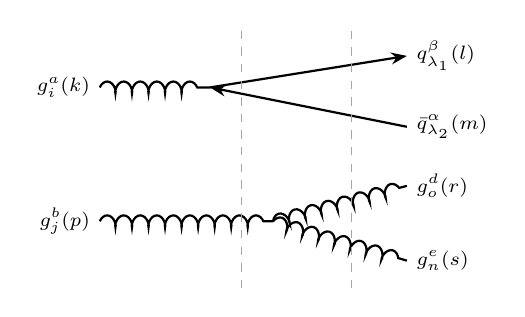
\begin{tikzpicture}
\draw[gl] (0,2.2) -- (1.4,2.2); \node[left] at (0,2.2) {\scriptsize$\gl{a}{i}{k}$};
\draw[qk] (1.4,2.2) -- (3.9,2.6); \node[right] at (3.9,2.6) {\scriptsize$\qk{\beta}{\lambda_{1}}{l}$};
\draw[qk] (3.9,1.7) -- (1.4,2.2); \node[right] at (3.9,1.7) {\scriptsize$\aqk{\alpha}{\lambda_{2}}{m}$};
\draw[gl] (0,0.5) -- (2.2,0.5); \node[left] at (0,0.5) {\scriptsize$\gl{b}{j}{p}$};
\draw[gl] (2.2,0.5) -- (3.9,0.95); \node[right] at (3.9,0.95) {\scriptsize$\gl{d}{o}{r}$};
\draw[gl] (2.2,0.5) -- (3.9,0.0); \node[right] at (3.9,0.0) {\scriptsize$\gl{e}{n}{s}$};
\draw[cut] (1.8,-0.35) -- (1.8,2.95); \draw[cut] (3.2,-0.35) -- (3.2,2.95);
\end{tikzpicture}
\end{center}
With $D_{1}=\eps_{k}-\eps_{l}-\eps_{m}$ and $D_{2}=\eps_{p}-\eps_{r}-\eps_{s}$ one has
$D_{1}+D_{2}=D_{f}$, and the two orderings telescope,
\begin{equation}
\frac{1}{D_{f}D_{1}}+\frac{1}{D_{f}D_{2}}=\frac{D_{1}+D_{2}}{D_{f}D_{1}D_{2}}=\frac{1}{D_{1}D_{2}},
\label{eq:partialfrac}
\end{equation}
so the final-state denominator cancels:
\begin{align}
\ket{\Psi^{ba}_{ji}(k,p)_{ggq\bar q}}=\frac{ig^{2}}{64\pi^{3}}\chg{27}
\sum\int\!d^{3}l\,d^{3}m\,d^{3}r\,d^{3}s\;
&\ket{q\bar q\,\gl{d}{o}{r}\gl{e}{n}{s}}\;t^{a}_{\beta\alpha}f^{bde}\,
\frac{\dthree(k-l-m)\dthree(p-r-s)}{\sqrt{k^{+}p^{+}r^{+}s^{+}}}
\nonumber\\&\times
\frac{\Ph^{i}_{\lambda_{1}\lambda_{2}}(k;l,m)\;\Vg^{jon}(p;r,s)}{D_{1}\,D_{2}}
+(k\leftrightarrow p)
\label{eq:Pggqq}
\end{align}
The topology in which one incoming gluon passes through untouched is disconnected --- it is
$\B_{3}$ with a spectator --- and does not belong here.\chg{28}

\subsubsection{Two quark--antiquark pairs outgoing}

Each gluon splits independently; both orderings again telescope by \eqref{eq:partialfrac}.
\begin{center}
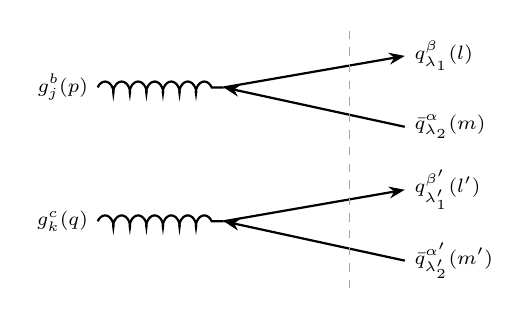
\begin{tikzpicture}
\draw[gl] (0,2.2) -- (1.6,2.2); \node[left] at (0,2.2) {\scriptsize$\gl{b}{j}{p}$};
\draw[qk] (1.6,2.2) -- (3.9,2.6); \node[right] at (3.9,2.6) {\scriptsize$\qk{\beta}{\lambda_{1}}{l}$};
\draw[qk] (3.9,1.7) -- (1.6,2.2); \node[right] at (3.9,1.7) {\scriptsize$\aqk{\alpha}{\lambda_{2}}{m}$};
\draw[gl] (0,0.5) -- (1.6,0.5); \node[left] at (0,0.5) {\scriptsize$\gl{c}{k}{q}$};
\draw[qk] (1.6,0.5) -- (3.9,0.9); \node[right] at (3.9,0.9) {\scriptsize$\qk{\beta'}{\lambda_{1}'}{l'}$};
\draw[qk] (3.9,0.0) -- (1.6,0.5); \node[right] at (3.9,0.0) {\scriptsize$\aqk{\alpha'}{\lambda_{2}'}{m'}$};
\draw[cut] (3.2,-0.35) -- (3.2,2.95);
\end{tikzpicture}
\end{center}
\begin{align}
\ket{\Psi^{cb}_{kj}(p,q)_{q\bar qq\bar q}}=\frac{g^{2}}{64\pi^{3}}\chg{29}
\sum\int\!d^{3}l\,d^{3}m\,d^{3}l'\,d^{3}m'\;
&\ket{q\bar q\,q\bar q}\;t^{b}_{\beta\alpha}t^{c}_{\beta'\alpha'}\,
\frac{\dthree(p-l-m)\dthree(q-l'-m')}{\sqrt{p^{+}q^{+}}}
\nonumber\\&\times
\frac{\Ph^{j}_{\lambda_{1}\lambda_{2}}(p;l,m)\;\Ph^{k}_{\lambda_{1}'\lambda_{2}'}(q;l',m')}
{\big(\eps_{p}-\eps_{l}-\eps_{m}\big)\big(\eps_{q}-\eps_{l'}-\eps_{m'}\big)}
\label{eq:Pqqqq}
\end{align}

%------------------------------------------------------------------
\subsection{Three-gluon incoming state}
%------------------------------------------------------------------
\subsubsection{One gluon, quark and antiquark outgoing}

One incoming gluon splits into $q\bar q$ while the other two merge into $\gl{e}{n}{s}$; both
orderings occur.
\begin{center}
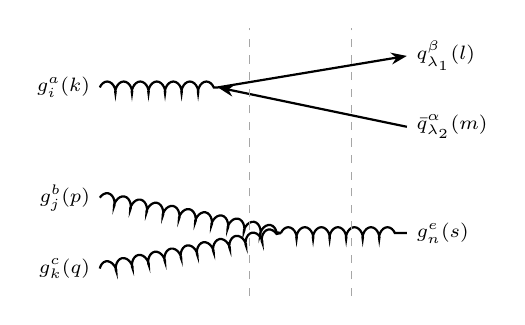
\begin{tikzpicture}
\draw[gl] (0,2.3) -- (1.5,2.3); \node[left] at (0,2.3) {\scriptsize$\gl{a}{i}{k}$};
\draw[qk] (1.5,2.3) -- (3.9,2.7); \node[right] at (3.9,2.7) {\scriptsize$\qk{\beta}{\lambda_{1}}{l}$};
\draw[qk] (3.9,1.8) -- (1.5,2.3); \node[right] at (3.9,1.8) {\scriptsize$\aqk{\alpha}{\lambda_{2}}{m}$};
\draw[gl] (0,0.9) -- (2.3,0.45); \node[left] at (0,0.9) {\scriptsize$\gl{b}{j}{p}$};
\draw[gl] (0,0.0) -- (2.3,0.45); \node[left] at (0,0.0) {\scriptsize$\gl{c}{k}{q}$};
\draw[gl] (2.3,0.45) -- (3.9,0.45); \node[right] at (3.9,0.45) {\scriptsize$\gl{e}{n}{s}$};
\draw[cut] (1.9,-0.35) -- (1.9,3.05); \draw[cut] (3.2,-0.35) -- (3.2,3.05);
\end{tikzpicture}
\end{center}
With $D_{A}=\eps_{k}-\eps_{l}-\eps_{m}$ (split first) and $D_{B}=\eps_{p}+\eps_{q}-\eps_{s}$
(merge first), $D_{A}+D_{B}=D_{f}$ and \eqref{eq:partialfrac} applies:
\begin{align}
\ket{\Psi^{cba}_{kji}(k,p,q)_{gq\bar q}}=-\frac{ig^{2}}{64\pi^{3}}
\sum\int\!d^{3}l\,d^{3}m\,d^{3}s\;
&\ket{q\bar q\,\gl{e}{n}{s}}\;t^{a}_{\beta\alpha}f^{ebc}\,
\frac{\dthree(k-l-m)\dthree(s-p-q)}{\sqrt{k^{+}s^{+}p^{+}q^{+}}}
\nonumber\\&\times
\frac{\Ph^{i}_{\lambda_{1}\lambda_{2}}(k;l,m)\;\Vg^{njk}(s;p,q)}{D_{A}\,D_{B}}
\label{eq:Pgqq}
\end{align}
summed over the \emph{three} inequivalent choices of which incoming gluon splits. Since
$f^{ebc}\Vg^{njk}(s;p,q)$ is symmetric under $(b,j,p)\leftrightarrow(c,k,q)$, summing over all six
permutations double counts.\chg{30}

%------------------------------------------------------------------
\subsection{Quark--antiquark incoming state}
%------------------------------------------------------------------
\subsubsection{Quark and antiquark outgoing}

Incoming $\qk{\beta'}{\lambda_{1}'}{l'}\aqk{\alpha'}{\lambda_{2}'}{m'}$, outgoing
$\qk{\beta}{\lambda_{1}}{l}\aqk{\alpha}{\lambda_{2}}{m}$, with
\begin{equation}
D_{f}\equiv\eps_{l'}+\eps_{m'}-\eps_{l}-\eps_{m}.
\end{equation}
Six diagrams contribute at $O(g^{2})$: the $s$-channel annihilation, the two time orderings of the
$t$-channel exchange, the instantaneous exchange between the two soft legs, and the two
instantaneous exchanges with the valence.\chg{36}

\paragraph{(a) $s$-channel: the pair annihilates into a gluon which splits again.}
\begin{center}
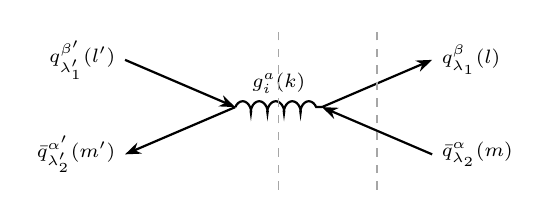
\begin{tikzpicture}
\draw[qk] (0,1.85) -- (1.4,1.25); \node[left] at (0,1.85) {\scriptsize$\qk{\beta'}{\lambda_{1}'}{l'}$};
\draw[qk] (1.4,1.25) -- (0,0.65); \node[left] at (0,0.65) {\scriptsize$\aqk{\alpha'}{\lambda_{2}'}{m'}$};
\draw[gl] (1.4,1.25) -- (2.5,1.25); \node[above] at (1.95,1.3) {\scriptsize$\gl{a}{i}{k}$};
\draw[qk] (2.5,1.25) -- (3.9,1.85); \node[right] at (3.9,1.85) {\scriptsize$\qk{\beta}{\lambda_{1}}{l}$};
\draw[qk] (3.9,0.65) -- (2.5,1.25); \node[right] at (3.9,0.65) {\scriptsize$\aqk{\alpha}{\lambda_{2}}{m}$};
\draw[cut] (1.95,0.2) -- (1.95,2.25); \draw[cut] (3.2,0.2) -- (3.2,2.25);
\end{tikzpicture}
\end{center}
\begin{equation}
\ket{\Psi^{1}_{q\bar q}}=\sum\int\! d^{3}k\,d^{3}l\,d^{3}m\;\ket{q\bar q}\;
\frac{\bra{\qk{\beta}{\lambda_{1}}{l}\aqk{\alpha}{\lambda_{2}}{m}}H_{gq\bar q}\ket{\gl{a}{i}{k}}}
{D_{f}}\;
\frac{\bra{\gl{a}{i}{k}}H_{gq\bar q}\ket{\qk{\beta'}{\lambda_{1}'}{l'}\aqk{\alpha'}{\lambda_{2}'}{m'}}}
{E_{q\bar q}(l',m')-E_{g}(k)}
\end{equation}
The second matrix element is the Hermitian conjugate of \eqref{eq:MEqqg}; using
$(t^{a}_{\beta'\alpha'})^{*}=t^{a}_{\alpha'\beta'}$ and $k=l+m=l'+m'$,
\begin{align}
\ket{\Psi^{1}_{q\bar q}}=\frac{g^{2}}{64\pi^{3}}\sum\int\!d^{3}l\,d^{3}m\;
&\ket{\qk{\beta}{\lambda_{1}}{l}\aqk{\alpha}{\lambda_{2}}{m}}\;
t^{a}_{\beta\alpha}t^{a}_{\alpha'\beta'}\;\dthree(l+m-l'-m')
\nonumber\\&\times
\frac{\Ph^{i}_{\lambda_{1}\lambda_{2}}(k;l,m)\,
\big[\Ph^{i}_{\lambda_{1}'\lambda_{2}'}(k;l',m')\big]^{*}\chg{31}}
{k^{+}\,\big(\eps_{l'}+\eps_{m'}-\eps_{k}\big)\,D_{f}}
\label{eq:E1a}
\end{align}
Note the two \emph{separate} spinor bilinears, the incoming one complex conjugated.

\paragraph{(b) $t$-channel: the quark emits, the antiquark absorbs.}
\begin{center}
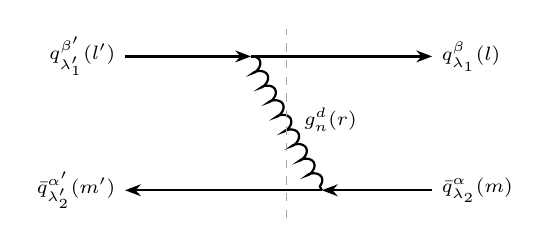
\begin{tikzpicture}
\draw[qk] (0,2.0) -- (1.6,2.0); \node[left] at (0,2.0) {\scriptsize$\qk{\beta'}{\lambda_{1}'}{l'}$};
\draw[qk] (1.6,2.0) -- (3.9,2.0); \node[right] at (3.9,2.0) {\scriptsize$\qk{\beta}{\lambda_{1}}{l}$};
\draw[qk] (3.9,0.3) -- (2.5,0.3); \node[right] at (3.9,0.3) {\scriptsize$\aqk{\alpha}{\lambda_{2}}{m}$};
\draw[qk] (2.5,0.3) -- (0,0.3); \node[left] at (0,0.3) {\scriptsize$\aqk{\alpha'}{\lambda_{2}'}{m'}$};
\draw[gl] (1.6,2.0) -- (2.5,0.3); \node[right] at (2.15,1.2) {\scriptsize$\gl{d}{n}{r}$};
\draw[cut] (2.05,-0.05) -- (2.05,2.35);
\end{tikzpicture}
\end{center}
With $r=l'-l$ (so $r^{+}>0$ requires $l'^{+}>l^{+}$) and $m=m'+r$, the intermediate state is
$\ket{\qk{\beta}{\lambda_{1}}{l}\gl{d}{n}{r}\aqk{\alpha'}{\lambda_{2}'}{m'}}$:
\begin{align}
\ket{\Psi^{2}_{q\bar q}}=\sum\int\! d^{3}r\,d^{3}l\,d^{3}m\;\ket{q\bar q}\;
&\frac{\bra{\aqk{\alpha}{\lambda_{2}}{m}}H_{gq\bar q}
\ket{\aqk{\alpha'}{\lambda_{2}'}{m'}\gl{d}{n}{r}}}{D_{f}}
\nonumber\\&\times
\frac{\bra{\qk{\beta}{\lambda_{1}}{l}\gl{d}{n}{r}}H_{gq\bar q}\ket{\qk{\beta'}{\lambda_{1}'}{l'}}}
{\eps_{l'}-\eps_{l}-\eps_{r}}
\end{align}
\begin{align}
\ket{\Psi^{2}_{q\bar q}}=-\frac{g^{2}}{64\pi^{3}}\sum\int\!d^{3}l\,d^{3}m\;
&\ket{\qk{\beta}{\lambda_{1}}{l}\aqk{\alpha}{\lambda_{2}}{m}}\;
t^{d}_{\beta\beta'}t^{d}_{\alpha'\alpha}\;\dthree(l+m-l'-m')
\nonumber\\&\times
\frac{\Ph^{n}_{\lambda_{1}\lambda_{1}'}(r;l,l')\,
\big[\Ph^{n}_{\lambda_{2}\lambda_{2}'}(r;m,m')\big]^{*}}
{r^{+}\,\big(\eps_{l'}-\eps_{l}-\eps_{r}\big)\,D_{f}},\qquad r=l'-l .
\label{eq:E1b}
\end{align}

\paragraph{(c) $t$-channel: the antiquark emits, the quark absorbs.}
\begin{center}
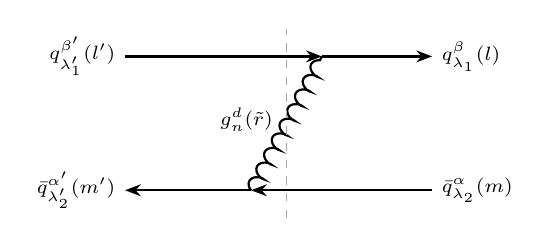
\begin{tikzpicture}
\draw[qk] (0,2.0) -- (2.5,2.0); \node[left] at (0,2.0) {\scriptsize$\qk{\beta'}{\lambda_{1}'}{l'}$};
\draw[qk] (2.5,2.0) -- (3.9,2.0); \node[right] at (3.9,2.0) {\scriptsize$\qk{\beta}{\lambda_{1}}{l}$};
\draw[qk] (3.9,0.3) -- (1.6,0.3); \node[right] at (3.9,0.3) {\scriptsize$\aqk{\alpha}{\lambda_{2}}{m}$};
\draw[qk] (1.6,0.3) -- (0,0.3); \node[left] at (0,0.3) {\scriptsize$\aqk{\alpha'}{\lambda_{2}'}{m'}$};
\draw[gl] (1.6,0.3) -- (2.5,2.0); \node[left] at (2.0,1.2) {\scriptsize$\gl{d}{n}{\tilde r}$};
\draw[cut] (2.05,-0.05) -- (2.05,2.35);
\end{tikzpicture}
\end{center}
Now $\tilde r=m'-m$ and $l=l'+\tilde r$; the intermediate state is
$\ket{\qk{\beta'}{\lambda_{1}'}{l'}\gl{d}{n}{\tilde r}\aqk{\alpha}{\lambda_{2}}{m}}$:
\begin{align}
\ket{\Psi^{3}_{q\bar q}}=-\frac{g^{2}}{64\pi^{3}}\sum\int\!d^{3}l\,d^{3}m\;
&\ket{\qk{\beta}{\lambda_{1}}{l}\aqk{\alpha}{\lambda_{2}}{m}}\;
t^{d}_{\beta\beta'}t^{d}_{\alpha'\alpha}\;\dthree(l+m-l'-m')
\nonumber\\&\times
\frac{\big[\Ph^{n}_{\lambda_{1}'\lambda_{1}}(\tilde r;l',l)\big]^{*}\,
\Ph^{n}_{\lambda_{2}'\lambda_{2}}(\tilde r;m',m)}
{\tilde r^{+}\,\big(\eps_{m'}-\eps_{m}-\eps_{\tilde r}\big)\,D_{f}},\qquad \tilde r=m'-m .
\label{eq:E1c}
\end{align}
Diagrams (b) and (c) populate complementary kinematic regions, $l'^{+}>l^{+}$ and
$l'^{+}<l^{+}$ respectively; together with (d) they build the full one-gluon exchange.

\paragraph{(d) Instantaneous gluon exchange between the two soft legs.\chg{37}}
\begin{center}
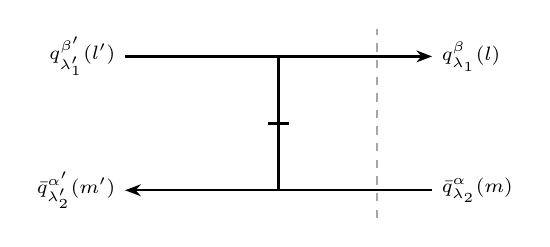
\begin{tikzpicture}
\draw[qk] (0,2.0) -- (3.9,2.0); \node[left] at (0,2.0) {\scriptsize$\qk{\beta'}{\lambda_{1}'}{l'}$};
\node[right] at (3.9,2.0) {\scriptsize$\qk{\beta}{\lambda_{1}}{l}$};
\draw[qk] (3.9,0.3) -- (0,0.3); \node[left] at (0,0.3) {\scriptsize$\aqk{\alpha'}{\lambda_{2}'}{m'}$};
\node[right] at (3.9,0.3) {\scriptsize$\aqk{\alpha}{\lambda_{2}}{m}$};
\draw[ins] (1.95,2.0) -- (1.95,0.3); \ibar{1.95}{1.15}
\draw[cut] (3.2,-0.05) -- (3.2,2.35);
\end{tikzpicture}
\end{center}
This is the $\Jc_{q}\!\cdot\!\Jc_{q}$ cross term; the exchanged line carries
$P^{+}=l'^{+}-l^{+}=m^{+}-m'^{+}$, and the product of a quark charge and an antiquark charge
carries one minus sign:
\begin{equation}
\ket{\Psi^{4}_{q\bar q}}=-\frac{g^{2}}{(2\pi)^{3}}\sum\int\!d^{3}l\,d^{3}m\;
\ket{q\bar q}\;
\frac{t^{a}_{\beta\beta'}t^{a}_{\alpha'\alpha}\,
\delta_{\lambda_{1}\lambda_{1}'}\delta_{\lambda_{2}\lambda_{2}'}\,\dthree(l+m-l'-m')}
{(l'^{+}-l^{+})^{2}\;D_{f}}
\label{eq:E1d}
\end{equation}

\paragraph{(e), (f) Instantaneous gluon exchange with the valence.}
\begin{center}
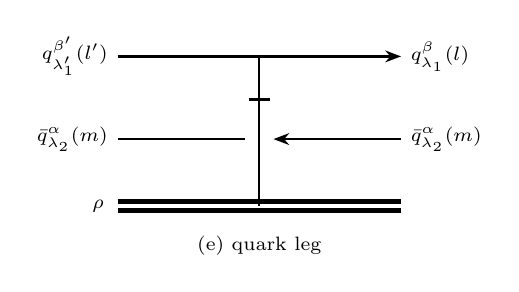
\begin{tikzpicture}
\draw[val] (0,0) -- (3.6,0); \node[left] at (-0.05,0) {\scriptsize$\rho$};
\draw[qk] (0,1.9) -- (3.6,1.9); \node[left] at (0,1.9) {\scriptsize$\qk{\beta'}{\lambda_{1}'}{l'}$};
\node[right] at (3.6,1.9) {\scriptsize$\qk{\beta}{\lambda_{1}}{l}$};
\draw[qk] (3.6,0.85) -- (1.98,0.85);
\draw[thick] (1.62,0.85) -- (0,0.85); \node[left] at (0,0.85) {\scriptsize$\aqk{\alpha}{\lambda_{2}}{m}$};
\node[right] at (3.6,0.85) {\scriptsize$\aqk{\alpha}{\lambda_{2}}{m}$};
\draw[ins] (1.8,0) -- (1.8,1.9); \ibar{1.8}{1.35}
\node at (1.8,-0.5) {\scriptsize (e) quark leg};
\end{tikzpicture}
\hspace{0.7cm}
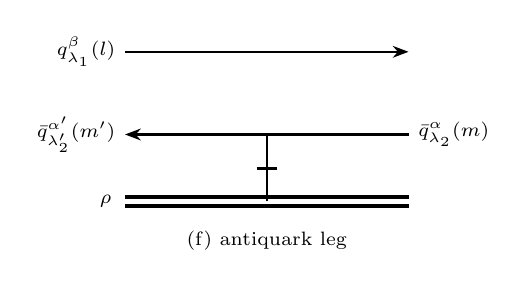
\begin{tikzpicture}
\draw[val] (0,0) -- (3.6,0); \node[left] at (-0.05,0) {\scriptsize$\rho$};
\draw[qk] (0,1.9) -- (3.6,1.9); \node[left] at (0,1.9) {\scriptsize$\qk{\beta}{\lambda_{1}}{l}$};
\draw[qk] (3.6,0.85) -- (0,0.85); \node[left] at (0,0.85) {\scriptsize$\aqk{\alpha'}{\lambda_{2}'}{m'}$};
\node[right] at (3.6,0.85) {\scriptsize$\aqk{\alpha}{\lambda_{2}}{m}$};
\draw[ins] (1.8,0) -- (1.8,0.85); \ibar{1.8}{0.42}
\node at (1.8,-0.5) {\scriptsize (f) antiquark leg};
\end{tikzpicture}
\end{center}
In (e) the antiquark is a spectator and the denominator is $\eps_{l'}-\eps_{l}$; in (f) the quark
is a spectator. The antiquark charge carries the extra minus sign of the current:
\begin{align}
\ket{\Psi^{5}_{q\bar q}}&=\frac{g^{2}}{(2\pi)^{3}}\sum\int\!d^{3}l\;\ket{q\bar q}\;
\frac{t^{a}_{\beta\beta'}\,\rho^{a}(l'-l)\,\delta_{\lambda_{1}\lambda_{1}'}\,
\delta^{\alpha\alpha'}\delta_{\lambda_{2}\lambda_{2}'}}
{(l'^{+}-l^{+})^{2}\,\big(\eps_{l'}-\eps_{l}\big)}
\label{eq:E1e}\\
\ket{\Psi^{6}_{q\bar q}}&=-\frac{g^{2}}{(2\pi)^{3}}\sum\int\!d^{3}m\;\ket{q\bar q}\;
\frac{t^{a}_{\alpha'\alpha}\,\rho^{a}(m'-m)\,\delta_{\lambda_{2}\lambda_{2}'}\,
\delta^{\beta\beta'}\delta_{\lambda_{1}\lambda_{1}'}}
{(m'^{+}-m^{+})^{2}\,\big(\eps_{m'}-\eps_{m}\big)}
\label{eq:E1f}
\end{align}
Diagrams (e) and (f) are the eikonal colour rotation of a soft quark in the valence background.
They populate the $b^{\dg}b$ and $d^{\dg}d$ structures, which the ansatz \eqref{eq:ansatz} does
not contain; within the $q\bar q$ sector they enter $\D_{3}$ through the spectator delta.

\subsubsection{Other outgoing states}

Two further sectors exist for a $q\bar q$ incoming state and are recorded for completeness.
At $O(g)$ the pair annihilates into a single gluon, which is the coefficient
$\A_{4}=-\A_{3}^{\dg}$ already fixed by unitarity. Also at $O(g)$, either member of the pair may
emit a gluon, $\ket{q\bar q}\to\ket{q\bar q\,g}$; the corresponding operator structures
$a^{\dg}b^{\dg}b$ and $a^{\dg}d^{\dg}d$ are \emph{absent} from the ansatz \eqref{eq:ansatz}.
They are generated by the same vertex \eqref{eq:MEqg} that produces $\A_{3}$ and are the quark
analogue of the three-gluon coefficient $C$; without them the $O(g)$ diagonalization cannot
cancel the matrix elements of $H_{gq\bar q}$ between $\ket{q\bar q}$ and $\ket{q\bar q\,g}$.

%==================================================================
\section{Coefficients of the evolution operator to $O(g^{2})$ through LCPT}
\label{sec:coeff}
%==================================================================

Applying the rule \eqref{eq:rule} to the wave functions of Sec.~\ref{sec:wf}.

\subsection{$\C_{0}$ and $\A_{1}$}
\begin{equation}
\C_{0}=1+O(g^{4}),\qquad
\C_{0}=1-\half\ip{l}\ip{m}\big[\A^{\alpha\beta}_{1\lambda_{2}\lambda_{1}}(m,l)\big]^{\dg}
\A^{\alpha\beta}_{1\lambda_{2}\lambda_{1}}(m,l)+O(g^{6})
\end{equation}
With $\A_{1}=(2\pi)^{3}\psi$, Eqs.~\eqref{eq:P1} and \eqref{eq:P2} give
\begin{equation}
\A^{\alpha\beta}_{1\lambda_{2}\lambda_{1}}(m,l)=
\frac{g^{2}t^{a}_{\beta\alpha}\rho^{a}(-k)\,k^{i}\Ph^{i}_{\lambda_{1}\lambda_{2}}(k;l,m)}
{2k^{+}k^{2}\eps_{q\bar q}}
-\frac{g^{2}t^{a}_{\beta\alpha}\rho^{a}(-k)\delta_{\lambda_{1}\lambda_{2}}}
{(k^{+})^{2}\eps_{q\bar q}} .\chg{33}
\end{equation}
Using $k^{i}\Gam^{i}(k;l,m)=4\eps_{k}-2\eps_{q\bar q}
-\tfrac{k^{+}}{l^{+}m^{+}}(\bm\sigma\!\cdot\!\bm l)(\bm\sigma\!\cdot\!\bm m)$, the instantaneous
term cancels the $\delta_{\lambda_{1}\lambda_{2}}$ piece \emph{exactly}:
\begin{res}
\begin{equation}
\boxed{\;
\A^{\alpha\beta}_{1\lambda_{2}\lambda_{1}}(m,l)=
-g^{2}t^{a}_{\beta\alpha}\rho^{a}(-k)\left[
\frac{\delta_{\lambda_{1}\lambda_{2}}}{k^{+}k^{2}}
+\frac{\chi^{\dg}_{\lambda_{1}}\big(\bm l\!\cdot\!\bm m+i(\bm l\!\times\!\bm m)\sigma^{3}\big)
\chi_{\lambda_{2}}}{2\,l^{+}m^{+}k^{2}\,\eps_{q\bar q}}\right]}
\label{eq:A1}
\end{equation}
$k=l+m$, $\bm l\!\times\!\bm m\equiv\epsilon^{ij}l^{i}m^{j}$. The cancellation is demanded by
unitarity: the right-hand side of the $\A_{2}$ relation contains no instantaneous piece.
\end{res}

\subsection{$\A_{3}$}
$\A_{3}=(2\pi)^{9/2}\psi$ with \eqref{eq:Pg}, and $(2\pi)^{9/2}/8\pi^{3/2}=(2\pi)^{3}/2\sqrt2$:
\begin{res}
\begin{equation}
\boxed{\;
\A^{a\alpha\beta}_{3i\lambda_{2}\lambda_{1}}(k,m,l)=
\frac{(2\pi)^{3}g\,t^{a}_{\beta\alpha}}{2\sqrt2\sqrt{k^{+}}}\;
\frac{\dthree(k-l-m)\;\Ph^{i}_{\lambda_{1}\lambda_{2}}(k;l,m)}{\eps_{k}-\eps_{l}-\eps_{m}}}
\label{eq:A3}
\end{equation}
\end{res}

\subsection{$\B_{3}$}
$\B_{3}=(2\pi)^{6}\psi_{\rm conn}$, and $(2\pi)^{6}/64\pi^{3}=(2\pi)^{3}/8$:
\begin{res}
\begin{equation}
\boxed{\;\B^{\alpha\beta ad}_{3\lambda_{2}\lambda_{1}in}(m,l,k,r)
=(2\pi)^{6}\Big[\psi_{\rm(a)}+\psi_{\rm(b)}+\psi_{\rm(c)}+\psi_{\rm(d)+(e)}
+\psi_{\rm(f)}+\psi_{\rm(g)}\Big]}
\label{eq:B3}
\end{equation}
where $\psi_{\rm(a)},\dots,\psi_{\rm(g)}$ are the coefficient functions of
Eqs.~\eqref{eq:B2a}, \eqref{eq:B2b}, \eqref{eq:B2c}, \eqref{eq:B2de}, \eqref{eq:B2f} and
\eqref{eq:B2g}. The prefactors become $(2\pi)^{3}g^{2}/8$ for (a), (b), (c);
$(2\pi)^{3}g^{2}/4$ for (d)+(e); $(2\pi)^{3}g^{2}/2$ for (f); and
$(2\pi)^{3}g^{2}/2$ for (g).
\end{res}

\subsection{$\B_{1}$}
$\B_{1}=(2\pi)^{6}\psi$, defined from the \emph{unsymmetrized} contribution (the exchange
$k\leftrightarrow p$ is supplied by Eq.~\eqref{eq:Omgg}):
\begin{res}
\begin{equation}
\boxed{\;\B^{ba\alpha\beta}_{1ji\lambda_{2}\lambda_{1}}(p,k,m,l)
=(2\pi)^{6}\Big[\psi_{\rm(a)}+\psi_{\rm(b1)}+\psi_{\rm(b2)}+\psi_{\rm(c)}+\psi_{\rm(d)}\Big]}
\label{eq:B1}
\end{equation}
where $\psi_{\rm(a)},\dots,\psi_{\rm(d)}$ are the coefficient functions of
Eqs.~\eqref{eq:C1a}, \eqref{eq:C1b1}, \eqref{eq:C1b2}, \eqref{eq:C1c} and \eqref{eq:C1d},
with prefactors $(2\pi)^{3}g^{2}/8$, $(2\pi)^{3}g^{2}/4$, $(2\pi)^{3}g^{2}/2$,
$(2\pi)^{3}g^{2}/2$ and $(2\pi)^{3}g^{2}/2$ respectively.
\end{res}

\subsection{$\C_{4}$, $\C_{3}$, $\D_{1}$: the factorized coefficients}

For these three sectors the transition proceeds through two independent subprocesses, the two
time orderings telescope by \eqref{eq:partialfrac}, and the coefficient factorizes into a product
of lower coefficients. With $\C_{4},\C_{3},\D_{1}=(2\pi)^{9}\psi$ and
$(2\pi)^{9}/64\pi^{3}=(2\pi)^{6}/8$:
\begin{res}
\begin{align}
\C^{bcde\alpha\beta}_{4jkon\lambda_{2}\lambda_{1}}(p,q,r,s,m,l)&=
\frac{i(2\pi)^{6}g^{2}}{8}t^{a}_{\beta\alpha}f^{bde}\,
\frac{\dthree(k-l-m)\dthree(p-r-s)}{\sqrt{k^{+}p^{+}r^{+}s^{+}}}
\nonumber\\&\hspace{1.1cm}\times
\frac{\Ph^{i}_{\lambda_{1}\lambda_{2}}(k;l,m)\,\Vg^{jon}(p;r,s)}
{\big(\eps_{k}-\eps_{l}-\eps_{m}\big)\big(\eps_{p}-\eps_{r}-\eps_{s}\big)}
\nonumber\\
&=\;\boxed{\;\A_{3}(k;m,l)\;C(p;r,s)\;}
\label{eq:C4}\\[8pt]
\C^{bcde\alpha\beta}_{3jkon\lambda_{2}\lambda_{1}}(p,q,r,s,m,l)&=
-\frac{i(2\pi)^{6}g^{2}}{8}t^{a}_{\beta\alpha}f^{ebc}\,
\frac{\dthree(k-l-m)\dthree(s-p-q)}{\sqrt{k^{+}s^{+}p^{+}q^{+}}}
\nonumber\\&\hspace{1.1cm}\times
\frac{\Ph^{i}_{\lambda_{1}\lambda_{2}}(k;l,m)\,\Vg^{njk}(s;p,q)}
{\big(\eps_{k}-\eps_{l}-\eps_{m}\big)\big(\eps_{p}+\eps_{q}-\eps_{s}\big)}
\nonumber\\
&=\;\boxed{\;\A_{3}(k;m,l)\;C^{\dg}(s;p,q)\;}
\label{eq:C3}\\[8pt]
\D^{cb\alpha'\beta'\alpha\beta}_{1kj\lambda_{2}'\lambda_{1}'\lambda_{2}\lambda_{1}}
(q,p,m',l',m,l)&=
\frac{(2\pi)^{6}g^{2}}{8}t^{b}_{\beta\alpha}t^{c}_{\beta'\alpha'}\,
\frac{\dthree(p-l-m)\dthree(q-l'-m')}{\sqrt{p^{+}q^{+}}}
\nonumber\\
&\hspace{1.2cm}\times
\frac{\Ph^{j}_{\lambda_{1}\lambda_{2}}(p;l,m)\Ph^{k}_{\lambda_{1}'\lambda_{2}'}(q;l',m')}
{\big(\eps_{p}-\eps_{l}-\eps_{m}\big)\big(\eps_{q}-\eps_{l'}-\eps_{m'}\big)}
\nonumber\\
&=\;\boxed{\,\A^{b\alpha\beta}_{3j\lambda_{2}\lambda_{1}}(p,m,l)\,
\A^{c\alpha'\beta'}_{3k\lambda_{2}'\lambda_{1}'}(q,m',l')\,}
\label{eq:D1}
\end{align}
\end{res}
\noindent
$C$ is the three-gluon coefficient of the pure Yang--Mills paper. The factorizations hold with no
leftover powers of $2\pi$, which is a stringent check on all four prefactors.

\subsection{$\D_{3}$}
From Eq.~\eqref{eq:Omqq}, $\D_{3}=-(2\pi)^{6}\psi$ with $\psi$ the coefficient function of the $s$-channel graph \eqref{eq:E1a}, the minus sign coming from the operator
ordering discussed after Eq.~\eqref{eq:ansatz}:
\begin{res}
\begin{equation}
\boxed{
\begin{aligned}
&\D^{\alpha'\beta'\alpha\beta}_{3\lambda_{2}'\lambda_{1}'\lambda_{2}\lambda_{1}}(m',l',m,l)
\Big|_{s\text{-ch}}
=-\frac{(2\pi)^{3}g^{2}}{8}\,t^{a}_{\beta\alpha}t^{a}_{\alpha'\beta'}\,\dthree(l+m-l'-m')
\\[3pt]
&\hspace{1.4cm}\times\;
\frac{\Ph^{i}_{\lambda_{1}\lambda_{2}}(k;l,m)\,
\big[\Ph^{i}_{\lambda_{1}'\lambda_{2}'}(k;l',m')\big]^{*}}
{k^{+}\big(\eps_{l'}+\eps_{m'}-\eps_{k}\big)\big(\eps_{l'}+\eps_{m'}-\eps_{l}-\eps_{m}\big)}
\end{aligned}}
\label{eq:D3res}
\end{equation}
\end{res}

\subsection{Closure checks}
\label{sec:checks}

The coefficients are over-determined; five independent checks are available and all pass.

\begin{enumerate}
\item[\bf 1.] \textbf{$\A_{1}$ against the $\A_{2}$ relation.} The instantaneous pieces enter
$\A_{1}$ and $\A_{2}$ with denominators $-\eps_{q\bar q}$ and $+\eps_{q\bar q}$ and cancel in the
sum. For the rest, using $4(k^{+})^{2}\eps_{k}=2k^{+}k^{2}$,
\[
\frac{1}{2k^{+}k^{2}\eps_{q\bar q}}+\frac{1}{4(k^{+})^{2}\eps_{q\bar q}(\eps_{q\bar q}-\eps_{k})}
=\frac{1}{2k^{+}k^{2}(\eps_{q\bar q}-\eps_{k})},
\]
which reproduces $\int_{p}\A_{3}(p,m,l)A^{b}_{j}(p)$ exactly, with
$A^{b}_{j}(p)=-\sqrt2 g p^{j}\rho^{b}(-p)/(\sqrt{p^{+}}p^{2})$.

\item[\bf 2.] \textbf{$\D_{1}$ against the $\D_{2}$ relation.} $\A_{3}$ contains no $\rho$, so
two $\A_{3}$'s commute and $\D_{1}^{\dg}=\A^{\dg}_{3}\A^{\dg}_{3}$. The $\D_{2}$ relation then
gives $\D_{2}=\A^{\dg}_{3}(q,m,l)\A^{\dg}_{3}(p,m',l')$ --- the crossed assignment, which is
exactly what direct LCPT gives for $\ket{q\bar qq\bar q}\to\ket{gg}$ (the reversed process has
denominators $-D_{1},-D_{2}$, whose signs cancel in $1/D_{1}D_{2}$). This check \emph{fixes} the
combinatorial factor: no other choice works.

\item[\bf 3.] \textbf{$\C_{4}$, $\C_{3}$ against their relations.} The factorized forms
$\C_{4}=\A_{3}C$ and $\C_{3}=\A_{3}C^{\dg}$ have precisely the operator content required by the
$\C_{2}$ and $\C_{1}$ relations.

\item[\bf 4.] \textbf{$\D_{3}$ against Eq.~\eqref{eq:U18}, and the sign.} Write
$D_{a}=\eps_{k}-\eps_{l}-\eps_{m}$, $D_{a}'=\eps_{k}-\eps_{l'}-\eps_{m'}$,
$D_{f}=\eps_{l'}+\eps_{m'}-\eps_{l}-\eps_{m}$, so $\eps_{l'}+\eps_{m'}-\eps_{k}=-D_{a}'$ and
$D_{a}-D_{a}'=D_{f}$. With $\D_{3}=s(2\pi)^{6}\psi$ the left-hand side of \eqref{eq:U18} is
\[
-s\frac{(2\pi)^{3}g^{2}}{8}\frac{t^{a}t^{a}\Ph\Ph^{*}\dthree}{k^{+}}
\Big[\frac{1}{D_{a}'D_{f}}-\frac{1}{D_{a}D_{f}}\Big]
=-s\frac{(2\pi)^{3}g^{2}}{8}\frac{t^{a}t^{a}\Ph\Ph^{*}\dthree}{k^{+}D_{a}D_{a}'},
\]
while the right-hand side is $+\tfrac{(2\pi)^{3}g^{2}}{8}t^{a}t^{a}\Ph\Ph^{*}\dthree/(k^{+}D_{a}D_{a}')$.
They agree if and only if $s=-1$, which is the sign in \eqref{eq:D3res}.

\item[\bf 5.] \textbf{$(2\pi)$ consistency.} The three factorizations \eqref{eq:C4}--\eqref{eq:D1}
hold with no leftover powers of $2\pi$ only if the prefactors
$(2\pi)^{3}/2\sqrt2$ and $(2\pi)^{6}/8$ are correct.
\end{enumerate}

%==================================================================
\section{Diagonalization of the Hamiltonian at $O(g)$}
\label{sec:diagg}
%==================================================================

\subsection{The similarity transformation order by order}

The evolution operator diagonalizes the soft Hamiltonian,
\begin{equation}
H_{\rm diag}=\OM^{\dg}H\,\OM=\sum_{n}E_{n}\ket{n}\bra{n},
\label{eq:Hdiag}
\end{equation}
and this is the second, equivalent characterization of $\OM$: the same operator that generates the
LCWF removes the off-diagonal matrix elements of $H$ between Fock sectors. It is convenient to
write $\OM=e^{iG}$ with $G=G_{1}+G_{2}+\dots$ Hermitian, so that
$\OM_{1}=iG_{1}$ is anti-Hermitian as required by unitarity, and
\begin{equation}
\OM^{\dg}H\OM=e^{-iG}He^{iG}
=H+\big[H,iG\big]+\frac{1}{2!}\Big[\big[H,iG\big],iG\Big]+\dots
\label{eq:BCH}
\end{equation}
Splitting the Hamiltonian by order in the coupling,
\begin{equation}
H=H_{0}+H^{(1)}+H^{(2)},\qquad
H^{(1)}=H_{g}+H_{ggg}+H_{gq\bar q},\qquad
H^{(2)}=H_{gggg}+H^{(A)}_{\rm inst}+H_{ggq\bar q},
\label{eq:Hsplit}
\end{equation}
and collecting powers of $g$ in \eqref{eq:BCH} gives
\begin{align}
O(g^{0}):&\qquad H_{0}
\label{eq:ord0}\\
O(g^{1}):&\qquad H^{(1)}+\big[H_{0},\OM_{1}\big]
\label{eq:ord1}\\
O(g^{2}):&\qquad H^{(2)}+\tfrac12\big[H^{(1)},\OM_{1}\big]+\big[H_{0},iG_{2}\big]
\label{eq:ord2}
\end{align}
where in \eqref{eq:ord2} we used $\big[[H_{0},\OM_{1}],\OM_{1}\big]=-[H^{(1)},\OM_{1}]$, which
follows once \eqref{eq:ord1} is imposed. Note that $iG_{2}$ and the normal ordered coefficient
$\OM_{2}$ of Sec.~\ref{sec:Omega} differ by $\tfrac12\OM_{1}^{2}$, since
$e^{iG}=1+iG_{1}+iG_{2}+\tfrac12(iG_{1})^{2}+\dots$; this is exactly the combination fixed by the
unitarity relation $\OM_{2}+\OM_{2}^{\dg}=\OM_{1}^{2}$. Both \eqref{eq:ord1} and \eqref{eq:ord2}
are manifestly Hermitian.

\subsection{The $O(g)$ condition}

Diagonality at $O(g)$ requires the whole of \eqref{eq:ord1} to vanish,
\begin{equation}
\boxed{\;\big[H_{0},\OM_{1}\big]=-H^{(1)}\;}
\label{eq:Ogcond}
\end{equation}
This is a strong statement: $H^{(1)}$ is \emph{purely} off-diagonal --- every term of
$H_{g}$, $H_{ggg}$ and $H_{gq\bar q}$ changes the Fock sector --- and $[H_{0},\cdot\,]$ is diagonal
in the operator basis, multiplying each normal ordered structure by its energy imbalance. Hence
\eqref{eq:Ogcond} can be solved structure by structure, and it \emph{determines} $\OM_{1}$
completely.

Writing the $O(g)$ Hamiltonian in Fock operator form,
\begin{align}
H_{g}&=\ip{p}\Big[\mathfrak a^{b}_{j}(p)\,a^{\dg b}_{j}(p)+\mathfrak a^{\dg b}_{j}(p)\,a^{b}_{j}(p)\Big],
&&\mathfrak a^{b}_{j}(p)=\frac{g\,p^{j}\rho^{b}(-p)}{\sqrt2\,(p^{+})^{3/2}},
\label{eq:Hgop}\\
H_{ggg}&=\ip{p}\ip{q}\ip{r}\Big[\mathfrak c(p;q,r)\,a^{\dg}_{r}a^{\dg}_{q}a_{p}+{\rm h.c.}\Big],
\\
H_{gq\bar q}&=\ip{p}\ip{l}\ip{m}\Big[\mathfrak v_{3}(p;m,l)\,b^{\dg}_{l}d^{\dg}_{m}a_{p}+{\rm h.c.}\Big]
\nonumber\\
&\quad+\ip{p}\ip{l'}\ip{l}\Big[\mathfrak v_{F}(p;l',l)\,a^{\dg}_{p}b^{\dg}_{l'}b_{l}+{\rm h.c.}\Big]
\nonumber\\
&\quad+\ip{p}\ip{m'}\ip{m}\Big[\mathfrak v_{G}(p;m',m)\,a^{\dg}_{p}d^{\dg}_{m'}d_{m}+{\rm h.c.}\Big],
\label{eq:Hqqgop}
\end{align}
the vertex functions are $(2\pi)^{9/2}$ times the matrix elements of Appendix~\ref{app:me}:
\begin{equation}
\mathfrak a=(2\pi)^{3/2}\bra{g}H_{g}\vac,\qquad
\mathfrak v_{3}=(2\pi)^{9/2}\bra{q\bar q}H_{gq\bar q}\ket{g},\qquad
\mathfrak v_{F}=(2\pi)^{9/2}\bra{q\,g}H_{gq\bar q}\ket{q},
\label{eq:vertexnorm}
\end{equation}
and similarly for $\mathfrak c$ and $\mathfrak v_{G}$, by the same counting as in
Eq.~\eqref{eq:rule}.

\subsection{Solution: the pure gauge structures}

With $[H_{0},a^{\dg}_{p}]=\eps_{p}a^{\dg}_{p}$ and
$[H_{0},a^{\dg}_{r}a^{\dg}_{q}a_{p}]=(\eps_{q}+\eps_{r}-\eps_{p})\,a^{\dg}_{r}a^{\dg}_{q}a_{p}$,
projecting \eqref{eq:Ogcond} onto the $a^{\dg}$ and $a^{\dg}a^{\dg}a$ structures gives
\begin{equation}
\eps_{p}A^{b}_{j}(p)+\mathfrak a^{b}_{j}(p)=0,
\qquad
(\eps_{q}+\eps_{r}-\eps_{p})\,C(p;q,r)+\mathfrak c(p;q,r)=0,
\end{equation}
so that
\begin{equation}
A^{b}_{j}(p)=-\frac{\mathfrak a^{b}_{j}(p)}{\eps_{p}}
=-\frac{\sqrt2\,g\,p^{j}\rho^{b}(-p)}{\sqrt{p^{+}}\,p^{2}},
\qquad
C(p;q,r)=\frac{\mathfrak c(p;q,r)}{\eps_{p}-\eps_{q}-\eps_{r}} .
\label{eq:ACfromdiag}
\end{equation}
The conjugate structures $a$ and $a^{\dg}aa$ are then fixed by the anti-Hermiticity of
$\OM_{1}$, and are cancelled automatically. These are precisely the Weizs\"acker--Williams and
three-gluon coefficients of the pure Yang--Mills paper.

\begin{res}
Equation~\eqref{eq:ACfromdiag} is worth pausing on: the diagonalization condition
\emph{derives} the $O(g)$ coefficients, rather than merely being consistent with them. Every
$O(g)$ coefficient is (vertex)/(energy denominator), which is the first-order LCPT expression ---
so the two characterizations of $\OM$, ``generates the LCWF'' and ``diagonalizes $H$'', agree
term by term at this order.
\end{res}

\subsection{Solution: the quark structures}

The quark--gluon vertex \eqref{eq:Hqqgop} contains three off-diagonal structures, and each
requires its own counterterm in $\OM_{1}$. Using
\begin{align}
\big[H_{0},\,b^{\dg}_{l}d^{\dg}_{m}a_{p}\big]&=(\eps_{l}+\eps_{m}-\eps_{p})\,b^{\dg}_{l}d^{\dg}_{m}a_{p},
\\
\big[H_{0},\,a^{\dg}_{p}b^{\dg}_{l'}b_{l}\big]&=(\eps_{p}+\eps_{l'}-\eps_{l})\,a^{\dg}_{p}b^{\dg}_{l'}b_{l},
\qquad
\big[H_{0},\,a^{\dg}_{p}d^{\dg}_{m'}d_{m}\big]=(\eps_{p}+\eps_{m'}-\eps_{m})\,a^{\dg}_{p}d^{\dg}_{m'}d_{m},
\end{align}
Eq.~\eqref{eq:Ogcond} gives
\begin{empheq}[box=\fbox]{align}
\A_{3}(p;m,l)&=\frac{\mathfrak v_{3}(p;m,l)}{\eps_{p}-\eps_{l}-\eps_{m}},
\label{eq:A3diag}\\
\mathcal F(p;l',l)&=\frac{\mathfrak v_{F}(p;l',l)}{\eps_{l}-\eps_{l'}-\eps_{p}},
\qquad
\mathcal G(p;m',m)=\frac{\mathfrak v_{G}(p;m',m)}{\eps_{m}-\eps_{m'}-\eps_{p}} .
\label{eq:FGdiag}
\end{empheq}
Using \eqref{eq:vertexnorm} and the matrix elements \eqref{eq:MEqqg}, \eqref{eq:MEqg},
\eqref{eq:MEaqg}, these read explicitly
\begin{align}
\A^{a\alpha\beta}_{3i\lambda_{2}\lambda_{1}}(k,m,l)&=
\frac{(2\pi)^{3}g\,t^{a}_{\beta\alpha}}{2\sqrt2\sqrt{k^{+}}}\,
\frac{\dthree(k-l-m)\,\Ph^{i}_{\lambda_{1}\lambda_{2}}(k;l,m)}{\eps_{k}-\eps_{l}-\eps_{m}},
\\
\mathcal F^{b\beta'\beta}_{j\lambda_{1}'\lambda_{1}}(p,l',l)&=
\frac{(2\pi)^{3}g\,t^{b}_{\beta'\beta}}{2\sqrt2\sqrt{p^{+}}}\,
\frac{\dthree(l-l'-p)\,\Ph^{j}_{\lambda_{1}'\lambda_{1}}(p;l',l)}{\eps_{l}-\eps_{l'}-\eps_{p}},
\label{eq:F}\\
\mathcal G^{b\alpha'\alpha}_{j\lambda_{2}'\lambda_{2}}(p,m',m)&=
-\frac{(2\pi)^{3}g\,t^{b}_{\alpha\alpha'}}{2\sqrt2\sqrt{p^{+}}}\,
\frac{\dthree(m-m'-p)\,\Ph^{j}_{\lambda_{2}\lambda_{2}'}(p;m,m')}{\eps_{m}-\eps_{m'}-\eps_{p}} .
\label{eq:G}
\end{align}
The first is the coefficient $\A_{3}$ of Sec.~\ref{sec:coeff}, reproduced exactly.

\begin{warn}
\textbf{The ansatz must be extended.} $\mathcal F$ and $\mathcal G$ --- gluon emission by a soft
quark and by a soft antiquark --- do not appear in the ansatz \eqref{eq:ansatz}. They are $O(g)$,
they are generated by the \emph{same} vertex \eqref{eq:Hqqgop} that produces $\A_{3}$, and
without them Eq.~\eqref{eq:Ogcond} has no solution: the $a^{\dg}b^{\dg}b$ and $a^{\dg}d^{\dg}d$
pieces of $H_{gq\bar q}$ would survive in $\OM^{\dg}H\OM$ and the Hamiltonian would not be
diagonal at $O(g)$. They are the quark analogue of the three-gluon coefficient $C$, and
\eqref{eq:ansatz} should be supplemented by
\begin{align}
&\ip{p}\ip{l'}\ip{l}\Big[\mathcal F(p;l',l)\,a^{\dg}_{p}b^{\dg}_{l'}b_{l}
-\mathcal F^{\dg}(p;l',l)\,b^{\dg}_{l}b_{l'}a_{p}\Big]
\nonumber\\
&\hspace{0.8cm}+\ip{p}\ip{m'}\ip{m}\Big[\mathcal G(p;m',m)\,a^{\dg}_{p}d^{\dg}_{m'}d_{m}
-\mathcal G^{\dg}(p;m',m)\,d^{\dg}_{m}d_{m'}a_{p}\Big].
\label{eq:FGansatz}
\end{align}
The unitarity relations of Sec.~\ref{sec:Omega} are unchanged by this addition except for the
$\D_{3}$ and $\B_{4}$ relations, which acquire the extra terms recorded in
Appendix~\ref{app:changelog}.\chg{39}
\end{warn}

\subsection{Result}

With $A$, $C$, $\A_{3}$, $\mathcal F$, $\mathcal G$ given by \eqref{eq:ACfromdiag},
\eqref{eq:A3diag} and \eqref{eq:FGdiag}, the whole of $H^{(1)}$ is cancelled and
\begin{res}
\begin{equation}
\boxed{\;\OM^{\dg}\big(H_{0}+H^{(1)}\big)\OM=H_{0}+O(g^{2})\;}
\label{eq:Ogresult}
\end{equation}
The soft Hamiltonian is \emph{completely} diagonalized at $O(g)$ --- not merely reduced to a
diagonal remainder. The free part survives untouched because the Weizs\"acker--Williams energy,
which is $O(g^{2})$ and $O(\rho^{2})$, has already been absorbed into the choice of $A$.
\end{res}

%==================================================================
\section{Diagonalization of the Hamiltonian at $O(g^{2})$}
\label{sec:diagg2}
%==================================================================

\subsection{What $\OM_{2}$ can and cannot remove}

At $O(g^{2})$ the transformed Hamiltonian is \eqref{eq:ord2},
\begin{equation}
\Big(\OM^{\dg}H\OM\Big)^{(2)}=\underbrace{H^{(2)}+\tfrac12\big[H^{(1)},\OM_{1}\big]}_{\textstyle \equiv\,\mathcal K}
+\big[H_{0},iG_{2}\big].
\label{eq:Kdef}
\end{equation}
For a normal ordered structure $\mathcal O$ whose creation operators carry total energy
$E_{\rm out}$ and annihilation operators $E_{\rm in}$,
\begin{equation}
\big[H_{0},\mathcal O\big]=\big(E_{\rm out}-E_{\rm in}\big)\,\mathcal O\equiv\Delta E\;\mathcal O .
\end{equation}
Therefore $iG_{2}$ can be chosen to cancel any piece of $\mathcal K$ with $\Delta E\neq0$, by
taking its coefficient to be $-\mathcal K/\Delta E$; and it can cancel \emph{nothing} with
$\Delta E=0$. The residual diagonal Hamiltonian is exactly the $\Delta E=0$ part of $\mathcal K$:
\begin{equation}
\boxed{\;H_{\rm diag}=H_{0}+\mathcal K\Big|_{\Delta E=0}\;}
\label{eq:residual}
\end{equation}
Two kinds of structure have $\Delta E=0$:
\begin{enumerate}
\item[(i)] the identity, $\mathcal O=\mathbf 1$ --- a $c$-number in the soft space, though an
operator in the valence space;
\item[(ii)] number-operator structures $a^{\dg}_{1}a_{2}$, $b^{\dg}b$, $d^{\dg}d$ whose
coefficient is supported at coinciding momenta, i.e.\ $\propto\dthree(p_{1}-p_{2})$.
\end{enumerate}
Everything else in $\mathcal K$ --- in particular every term carrying an explicit $\rho$, which
transfers momentum to the soft sector and therefore has $\Delta E\neq0$ away from a set of
measure zero --- is removed by $iG_{2}$. We take the two surviving classes in turn.

\subsection{The identity: the background field energy}

The only term of $\mathcal K$ with all soft operators contracted is the one in which a gluon is
emitted by $\rho$ and reabsorbed by $\rho$,
\begin{equation}
\tfrac12\big[H_{g},\OM_{1}\big]\Big|_{\mathbf 1}
=\tfrac12\ip{p}\Big[\mathfrak a^{\dg b}_{j}(p)A^{b}_{j}(p)+A^{\dg b}_{j}(p)\mathfrak a^{b}_{j}(p)\Big]
=-\ip{p}\frac{\mathfrak a^{\dg b}_{j}(p)\,\mathfrak a^{b}_{j}(p)}{\eps_{p}},
\end{equation}
using $A=-\mathfrak a/\eps_{p}$ from \eqref{eq:ACfromdiag}. The corresponding quark term vanishes:
$H_{gq\bar q}$ creates a $q\bar q$ pair and $\OM_{1}$ must then annihilate it, which leaves an
uncontracted $a^{\dg}a$ rather than the identity --- pair creation out of the vacuum is
$O(g^{2})$, so its square is $O(g^{4})$. Likewise $H_{ggg}$ contributes nothing at this order.
Inserting $\mathfrak a^{b}_{j}(p)=g\,p^{j}\rho^{b}(-p)/\sqrt2\,(p^{+})^{3/2}$ and
$\eps_{p}=p^{2}/2p^{+}$,
\begin{res}
\begin{equation}
\mathcal K\Big|_{\mathbf 1}
=-\ip{p}\frac{g^{2}\,\rho^{b}(p)\,\rho^{b}(-p)}{(p^{+})^{2}}
\;=\;-\ip{p}\eps_{p}\,A^{\dg b}_{j}(p)A^{b}_{j}(p) .
\label{eq:WW}
\end{equation}
\end{res}
\noindent
This is the coherent Weizs\"acker--Williams background field energy. It is the \emph{only}
surviving correction, and its form is unchanged from the pure Yang--Mills case --- but
$\rho=\rho_{g}+\rho_{q}$ now includes the fundamental representation charge of the valence
quarks, Eq.~\eqref{eq:rho}. That is the whole of the quark modification to the ground state energy
at this order.

\subsection{The gluon number operator: gluon and quark loops}

The $a^{\dg}_{1}a_{2}$ part of $\mathcal K$ receives contributions from $H_{ggg}\times C$ and
from $H_{gq\bar q}\times\A_{3}$, together with $\rho$-dependent pieces of $H^{(2)}$ and of
$H_{g}\times C$. The latter carry explicit $\rho$ and are removed by $iG_{2}$. The former two are
momentum diagonal and survive. Writing them together,
\begin{align}
\mathcal K\Big|_{a^{\dg}a,\,\Delta E=0}
&=\ip{p}a^{\dg}_{p}a_{p}\Big[\underbrace{2\!\!\int\limits_{q,r}\!\!\big(\eps_{q}+\eps_{r}-\eps_{p}\big)
C^{\dg}(p;q,r)C(p;q,r)}_{\text{gluon loop}}
\nonumber\\
&+\underbrace{\int\limits_{\kappa,\bar\kappa}\!\big(\eps_{\kappa}+\eps_{\bar\kappa}-\eps_{p}\big)
\A^{\dg}_{3}(p;\kappa\bar\kappa)\A_{3}(p;\kappa\bar\kappa)}_{\text{quark loop}}\Big],
\label{eq:loops}
\end{align}
each being $-\!\int|{\rm vertex}|^{2}/({\rm energy\ denominator})$, i.e.\ the second-order
light-cone energy shift of a single soft gluon.

Both vanish. Introduce, for the splitting $p\to$ two quanta with longitudinal fractions $z$ and
$1-z$, the relative transverse momentum $\bm\kappa$ of Eq.~\eqref{eq:kappa}. The measure is
$d^{3}l=p^{+}dz\,d^{2}\kappa$, the energy denominator is
$\eps_{p}-\eps_{l}-\eps_{m}=-\kappa^{2}/2z(1-z)p^{+}$, and for the quark loop the spin and colour
sums give, using \eqref{eq:kappa},
\begin{equation}
\sum_{\lambda_{1}\lambda_{2}}\sum_{i}\big|\Ph^{i}_{\lambda_{1}\lambda_{2}}(p;l,m)\big|^{2}
=\frac{4\,\kappa^{2}\big[z^{2}+(1-z)^{2}\big]}{(p^{+})^{2}z^{2}(1-z)^{2}} .
\end{equation}
Every power of $\kappa$ then cancels between numerator and denominator and one is left with
\begin{equation}
\text{quark loop}\;\propto\;g^{2}N_{f}T_{F}\int_{\Lam/p^{+}}^{1-\Lam/p^{+}}\!\!dz\;
\frac{z^{2}+(1-z)^{2}}{z(1-z)}\;\int\! d^{2}\kappa ,
\label{eq:scaleless}
\end{equation}
and similarly for the gluon loop with $z^{2}+(1-z)^{2}$ replaced by the gluonic splitting
function. The transverse integral carries no scale --- the soft gluon is massless and there is no
external invariant --- so it vanishes in dimensional regularization, as does the
$\int d^{2}\kappa/\kappa^{2}$ that appears in the corresponding norm.
\begin{res}
\begin{equation}
\mathcal K\Big|_{a^{\dg}a,\,\Delta E=0}=0 .
\label{eq:loopzero}
\end{equation}
This is the statement that a free massless gluon receives no mass correction, as gauge invariance
requires. It holds separately for the gluon loop and for the quark loop, and it is the reason the
$N_{f}$ dependence does not appear in the diagonalized Hamiltonian at this order.
\end{res}

\subsection{The quark number operators}

The $b^{\dg}b$ and $d^{\dg}d$ parts of $\mathcal K$ come from two places. The $\rho$-dependent
ones --- the instantaneous $\rho\!\cdot\!\Jc_{q}$ exchange of Eqs.~\eqref{eq:E1e},
\eqref{eq:E1f}, and the products $H_{g}\times\mathcal F$, $H_{g}\times\mathcal G$ --- describe the
eikonal colour rotation of a soft quark in the valence field. They transfer momentum to the soft
quark, so $\Delta E=\eps_{l'}-\eps_{l}\neq0$ and they are removed by $iG_{2}$. What remains is the
momentum-diagonal self-energy,
\begin{equation}
\mathcal K\Big|_{b^{\dg}b,\,\Delta E=0}
=\ip{l}\int\limits_{p,l'}\big(\eps_{p}+\eps_{l'}-\eps_{l}\big)
\mathcal F^{\dg}(p;l',l)\mathcal F(p;l',l)\;b^{\dg}_{l}b_{l},
\end{equation}
which is again $-\!\int|{\rm vertex}|^{2}/({\rm denominator})$ for a massless on-shell quark and
therefore proportional to the same scaleless transverse integral as \eqref{eq:scaleless}. It
vanishes, and so does the $d^{\dg}d$ term.

\subsection{Result}

Collecting \eqref{eq:residual}, \eqref{eq:WW}, \eqref{eq:loopzero} and the vanishing of the quark
number terms,
\begin{res}
\begin{equation}
\boxed{\;
\OM^{\dg}H\,\OM=H_{0}-\ip{p}\frac{g^{2}\,\rho^{a}(p)\,\rho^{a}(-p)}{(p^{+})^{2}}
\;+\;O(g^{3}),\qquad \rho^{a}=\rho^{a}_{g}+\rho^{a}_{q}\;}
\label{eq:g2result}
\end{equation}
\end{res}

\noindent
Three remarks.

\paragraph{The quark sector adds no new diagonal structure.} Every quark induced term at
$O(g^{2})$ is either removable by $iG_{2}$ --- because it carries an explicit $\rho$ and so
transfers momentum --- or proportional to a scaleless integral. The sole quark modification of
\eqref{eq:g2result} is that $\rho$ now contains the valence quark charge density $\rho_{q}$. The
form of the background field energy, and the fact that it is the only survivor, are unchanged
from pure Yang--Mills.

\paragraph{Consistency with the coefficients of Sec.~\ref{sec:coeff}.} The $O(g)$ condition
\eqref{eq:Ogcond} reproduced $A$, $C$, $\A_{3}$ and gave $\mathcal F$, $\mathcal G$; the $O(g^{2})$
construction requires $iG_{2}$ to cancel the off-diagonal part of $\mathcal K$, which is the
same information carried by the $O(g^{2})$ coefficients $\A_{1}$, $\B_{1}$, $\B_{3}$, $\C_{3}$,
$\C_{4}$, $\D_{1}$, $\D_{3}$ obtained by LCPT matching. The two routes are the same calculation
read in opposite directions, and the closure checks of Sec.~\ref{sec:checks} are what verifies
that they agree.

\paragraph{Why $N_{f}$ is absent.} One might have expected a quark loop contribution
$\propto\alpha_{s}N_{f}$ in the diagonalized Hamiltonian, since that is where the $N_{f}$ part of
the running coupling comes from. It is absent here because \eqref{eq:g2result} is the energy of
the \emph{soft} sector in a fixed valence background, with the soft gluon strictly on shell and
massless. The $N_{f}$ dependence enters physical quantities through the evolution of
$\rho$ and through the $O(g^{3})$ and $O(g^{4})$ coefficients of $\OM$, not through the
$O(g^{2})$ ground state energy.


\appendix
%==================================================================
\section{Matrix elements}
\label{app:me}
%==================================================================
\begin{align}
\bra{\gl{a}{i}{k}}H_{g}\vac&=\frac{g\,k^{i}\rho^{a}(-k)}{4\pi^{3/2}|k^{+}|^{3/2}}
\label{eq:MEg}\\
\bra{\gl{c}{l}{q}\gl{b}{j}{p}}H_{g}\ket{\gl{a}{i}{k}}&=
\delta^{ac}\delta_{il}\dthree(k-q)\frac{g\,p^{j}\rho^{b}(-p)}{4\pi^{3/2}|p^{+}|^{3/2}}
+\big(b,j,p\leftrightarrow c,l,q\big)
\label{eq:MEg2}\\
\bra{\gl{c}{l}{q}\gl{b}{j}{p}}H_{ggg}\ket{\gl{a}{i}{k}}&=
\frac{igf^{abc}\dthree(k-p-q)}{8\pi^{3/2}\sqrt{k^{+}p^{+}q^{+}}}\Vg^{ijl}(k;p,q)
\label{eq:MEggg}\\
\bra{\qk{\beta}{\lambda_{1}}{l}\aqk{\alpha}{\lambda_{2}}{m}}H_{gq\bar q}\ket{\gl{a}{i}{k}}&=
\frac{g\,t^{a}_{\beta\alpha}}{8\pi^{3/2}\sqrt{k^{+}}}\dthree(k-l-m)
\Ph^{i}_{\lambda_{1}\lambda_{2}}(k;l,m)
\label{eq:MEqqg}\\
\bra{\qk{\beta'}{\lambda_{1}'}{l'}\gl{d}{n}{r}}H_{gq\bar q}\ket{\qk{\beta}{\lambda_{1}}{l}}&=
\frac{g\,t^{d}_{\beta'\beta}}{8\pi^{3/2}\sqrt{r^{+}}}\dthree(l-l'-r)
\Ph^{n}_{\lambda_{1}'\lambda_{1}}(r;l',l)
\label{eq:MEqg}\\
\bra{\aqk{\alpha'}{\lambda_{2}'}{m'}\gl{d}{n}{r}}H_{gq\bar q}\ket{\aqk{\alpha}{\lambda_{2}}{m}}&=
-\frac{g\,t^{d}_{\alpha\alpha'}}{8\pi^{3/2}\sqrt{r^{+}}}\dthree(m-m'-r)
\Ph^{n}_{\lambda_{2}\lambda_{2}'}(r;m,m')
\label{eq:MEaqg}\\
\bra{\qk{\beta}{\lambda_{1}}{l}\aqk{\alpha}{\lambda_{2}}{m}}H_{q\bar q-\rm inst}\vac&=
\frac{g^{2}t^{a}_{\beta\alpha}\rho^{a}(-l-m)\delta_{\lambda_{1}\lambda_{2}}}
{8\pi^{3}(l^{+}+m^{+})^{2}}
\label{eq:MEinst}\\
\bra{\qk{\beta}{\lambda_{1}}{l}\aqk{\alpha}{\lambda_{2}}{m}}H_{ggq\bar q}\ket{\gl{a}{i}{k}\gl{b}{j}{p}}&=
\frac{g^{2}\dthree(k+p-l-m)}{16\pi^{3}\sqrt{k^{+}p^{+}}}
\chi^{\dg}_{\lambda_{1}}\!\Big[\frac{(t^{a}t^{b})_{\beta\alpha}\sigma^{i}\sigma^{j}}{l^{+}-k^{+}}
+\frac{(t^{b}t^{a})_{\beta\alpha}\sigma^{j}\sigma^{i}}{l^{+}-p^{+}}\Big]\chi_{\lambda_{2}}
\end{align}
The instantaneous fermion line carries $1/(2P^{+}_{\rm inst})$, $P^{+}_{\rm inst}$ being the $+$
momentum flowing along it.

%==================================================================
\section{Change log}
\label{app:changelog}
%==================================================================

\begin{center}
\renewcommand{\arraystretch}{1.15}\small
\begin{longtable}{c>{\raggedright\arraybackslash}p{3.9cm}p{7.6cm}}
\hline
\# & previous form & change and reason\\
\hline
\endhead
C0 & --- & Conventions subsection added: vertex function $\Gam^{i}$, label assignment, the
$(2\pi)$ matching rule. Everything below is checkable mechanically once these are fixed.\\
C1 & $\A_{4}(p)$ & arguments restored to $(l,m,p)$, per the right-to-left rule.\\
C2 & $\B_{2}(l,m,p,q)$, $\B_{4}(m,l,p,q)$ & $\to(l,m,q,p)$ and $(q,p,l,m)$.\\
C3 & $\C^{\ldots\beta\alpha}_{4\ldots\lambda_{1}\lambda_{2}}(\ldots,l,m)$ &
$\to\C^{\ldots\alpha\beta}_{4\ldots\lambda_{2}\lambda_{1}}(\ldots,m,l)$, matching $\C_{3}$.\\
C4 & $a^{c}_{k}(q)$ in $\D_{2}$ & $\to a^{\dg c}_{k}(q)$: the conjugate of $\D_{1}$ creates two
gluons. As printed the term also violated $O(g^{2})$ counting.\\
C5 & --- & The $\D_{3}$ pair is annihilated as $b(l')d(m')$ while every other term uses $d\,b$;
this produces the explicit minus signs in Eqs.~\eqref{eq:Omqq} and \eqref{eq:D3res}.
Verified by closure check 4.\\
C6 & no prefactor & $(2\pi)^{3}$ inserted in $\OM\vac$. From \eqref{eq:rule} with $(n,M)=(0,2)$.
This is why the previous $\A_{1}$ carried $(2\pi)^{6}$ instead of $(2\pi)^{3}$.\\
C7 & $\ket{\aqk{\beta}{\lambda_{1}}{l}\qk{\alpha}{\lambda_{2}}{m}}$ & quark and antiquark
interchanged relative to the ansatz and to $\OM\ket{g}$. Corrected here and, consequently, in all
of Sec.~\ref{sec:coeff}.\\
C8 & $(2\pi)^{3/2}$ & $\to(2\pi)^{3}$ for the $\B_{3}$ term: $(n,M)=(1,3)$.\\
C9 & single term & symmetrization over the two incoming gluons restored, as in Eq.~(4.17) of the
pure Yang--Mills paper.\\
C10 & --- & disconnected components ($\A_{1}$, $\A_{3}$, $\B_{3}$ with spectators) added
explicitly; they must be subtracted before reading off $\B_{1}$, $\C_{4}$, $\C_{3}$.\\
C11 & $(l,m)$ used for both & incoming labels changed to $(l',m')$; the integration and the
outgoing state carry $(l,m)$, matching the ansatz.\\
C12 & $\A_{4\lambda_{1}\lambda_{2}b}$, $\A^{\dg}_{3j\lambda_{1}\lambda_{2}}$ &
$\to\A_{4\lambda_{1}\lambda_{2}j}$ and $\A^{\dg}_{3j\lambda_{2}\lambda_{1}}$.\\
C13 & $C^{b'cb}_{j'kj}$ & $\to C^{\dg b'cb}_{j'kj}$: the term comes from
$(-C^{\dg}a^{\dg}aa)(-\A^{\dg}_{3}a^{\dg}db)$, so $C$ is necessarily daggered.\\
C14 & $\C_{1,2}^{\beta\alpha abcde}$ & stray superscript $a$ removed.\\
C15 & $\A^{b\alpha\beta\dg}_{j\lambda_{2}\lambda_{1}}$ & subscript $3$ restored.\\
C16 & $\D^{\dg}_{3}(m',l',m,l)$ & $\to\D^{\dg}_{3}(m,l,m',l')$: conjugating and restoring the
standard operator order relabels $l\leftrightarrow l'$, $m\leftrightarrow m'$.\\
C17 & $\big(\tfrac{p^{2}}{2p^{+}}+\tfrac{q^{2}}{2q^{+}}\big)$ &
$\to\eps_{k}-\eps_{l}-\eps_{m}$. The defining equation already had
$E_{g}(k)-E_{q\bar q}$; the explicit form dropped $\eps_{k}$ and flipped the signs. Propagated
into the previous $\A_{3}$.\\
C18 & $\sigma^{l}(\bm\sigma\!\cdot\!\bm q)/q^{+}$ & the last slot of $\Gam$ must carry the
\emph{incoming quark} momentum $p$ (resp.\ the outgoing antiquark $m'$), not the antiquark
momentum $q$.\\
C19 & --- & missing diagram: $g\to gg$ through $H_{ggg}$ followed by $g\to q\bar q$.\\
C20 & --- & missing time ordering: the valence emits $r$ \emph{first} (denominator $-\eps_{r}$).\\
C21 & --- & missing diagram: instantaneous quark exchange $\bra{q\bar q g}H_{ggq\bar q}\ket{g}$.\\
C22 & counted as a contribution & the topology with a spectator incoming gluon is disconnected and
belongs to $\A_{1}$.\\
C23 & $1/\sqrt{k^{+}p^{+}q'^{+}}$ & $\to 1/(q'^{+}\sqrt{k^{+}p^{+}})$: the second vertex supplies
a further $1/\sqrt{q'^{+}}$.\\
C24 & $\eps_{k}-\eps_{p}-\eps_{q}-\eps_{r}$ & $\to\eps_{k}+\eps_{p}-\eps_{q}-\eps_{r}$:
$E_{\rm in}=\eps_{k}+\eps_{p}$.\\
C25 & $g^{2}/32\pi^{3}$ & $\to g^{2}/16\pi^{3}$: the intermediate denominator $\eps_{k}$
contributes $2k^{+}/k^{2}$.\\
C26 & --- & missing diagram: instantaneous $\bra{q\bar q}H_{ggq\bar q}\ket{gg}$.\\
C27 & $g^{2}/128\pi^{3}$, one ordering & $\to g^{2}/64\pi^{3}$ (the $\tfrac12$ cancels against the
two assignments of identical gluons, as in Eqs.~(4.56)--(4.57) of the pure Yang--Mills paper), and
the second time ordering added --- which is what makes the result factorize.\\
C28 & counted as $\C_{4}$ & the topology with $\dthree(u-p)\delta^{bf}\delta_{jn}$ has a spectator
gluon: it is $\B_{3}$ disconnected, not $\C_{4}$.\\
C29 & $g^{2}/128\pi^{3}$, one ordering, denominator missing $+\eps_{p}$ & corrected; both
orderings added, giving the factorized form.\\
C30 & six permutations & three inequivalent assignments: $f^{ebc}\Vg^{njk}(s;p,q)$ is symmetric
under $(b,j,p)\leftrightarrow(c,k,q)$, so six double counts.\\
C31 & $\chi^{\dg}(\cdots)\chi^{\dg}\chi(\cdots)\chi$ & malformed spinor string replaced by two
separate bilinears with the incoming one conjugated; the trailing $+(p\leftrightarrow q)$ removed
($p$, $q$ are the quark and antiquark, not identical particles).\\
C32 & --- & $t$-channel and instantaneous $\mathcal J_{q}\!\cdot\!\mathcal J_{q}$ exchange noted
as still to be computed, with the constraint they must satisfy.\\
C33 & $(2\pi)^{6}$, $t^{a}_{\alpha\beta}$, $\chi^{\dg}_{\lambda_{2}}\!\cdots\chi_{\lambda_{1}}$ &
$(2\pi)^{3}$ (see C6) and the labels of \eqref{eq:qlabels} (see C7); compact form
\eqref{eq:A1} derived.\\
C34 & compact $\psi$'s only & Sec.~\ref{sec:wf} rewritten in full: every contribution now carries
its diagram, its formal LCPT expression with matrix elements and energy denominators displayed,
and the evaluated result --- the level of detail of the vacuum sector in the original draft.\\
C35 & --- & new diagrams: the $\Jc_{q}\!\cdot\!\Jc_{g}$ instantaneous gluon exchange, in the
$\B_{3}$ sector, Eq.~\eqref{eq:B2g}, and in the $\B_{1}$ sector, Eq.~\eqref{eq:C1d}. These arise
because the soft gluon charge density can be contracted against the soft quark current, not only
against $\rho$; they appear nowhere in the previous drafts.\\
C36 & $s$-channel only & the $q\bar q\to q\bar q$ sector now carries all six diagrams:
$s$-channel, the two time orderings of the $t$-channel exchange, the instantaneous
$\Jc_{q}\!\cdot\!\Jc_{q}$ exchange, and the two instantaneous exchanges with the valence.\\
C37 & --- & the $t$-channel orderings (b) and (c) populate the complementary kinematic regions
$l'^{+}\gtrless l^{+}$; with the instantaneous graph (d) they build the full one-gluon exchange.\\
C39 & --- & Secs.~\ref{sec:diagg} and \ref{sec:diagg2} written. The $O(g)$ condition
$[H_{0},\OM_{1}]=-H^{(1)}$ \emph{derives} $A$, $C$ and $\A_{3}$, and forces two further $O(g)$
coefficients $\mathcal F$, $\mathcal G$ (gluon emission by a soft quark or antiquark) that the
ansatz \eqref{eq:ansatz} does not contain; without them the Hamiltonian is not diagonal at
$O(g)$. See Eq.~\eqref{eq:FGansatz}.\\
C40 & --- & the valence charge density is written as $\rho=\rho_{g}+\rho_{q}$,
Eq.~\eqref{eq:rho}. This is the only way the quark sector modifies the diagonalized Hamiltonian
at $O(g^{2})$, Eq.~\eqref{eq:g2result}.\\
C38 & --- & $H^{(A)}_{\rm inst}$ written as a single current--current operator,
Eq.~\eqref{eq:HinstA}. Expanding $\Jc=\rho+\Jc_{g}+\Jc_{q}$ makes the enumeration of
instantaneous contributions exhaustive; this is what exposed C35.\\
\hline
\end{longtable}
\end{center}

\noindent
Unchanged and correct as previously written: $\C_{0}=1$; the $\A_{2}$, $\B_{2}$ relations; the
$\A_{1}$ term of $\OM\ket{g}$ and the $\A_{3}$, $\C_{4}$, $\D_{1}$, $\C_{3}$, $\D_{3}$ prefactors
in the action-on-states equations; and the prefactor $(2\pi)^{3}g/2\sqrt2$ of $\A_{3}$.

\end{document}
